\documentclass[master]{finthesis}

\usepackage{anyfontsize}
\usepackage{subcaption}
\usepackage{tikz}
\usetikzlibrary{arrows.meta}
\usetikzlibrary{through, patterns}
\usetikzlibrary{positioning}
\usepackage{float} 
\usepackage{caption}
\usepackage{url}
\usepackage{url}
\usepackage{amsmath}
\usepackage{fancyvrb}
\usepackage{amssymb}
\usepackage{fix-cm}
\usepackage{multicol}

\addbibresource{main.bib}

\title{Систем за препознавање гестикулација шаком на видео снимцима са веб камере коришћењем модела дубоког учења}
\author{Ана Ђ. Јовановић}
\studid{396/2024}
\advisor{проф. др Владимир М. Миловановић}
\advisorfull{Др Владимир М. Миловановић,\\ванредни професор}

\studprog{Електротехника и рачунарство}
% \module{Модул}
\course{Анализа и пројектовање алгоритама}
% \date{\today}
\date{2026-02-10}

\committee{проф. др Јасна Радуловић}
\committee{проф. др Петар Тодоровић}

\studentshould{% У оквиру овог рада кандидат треба да...
    реализује систем за препознавање шаке и гестикулација шаком у
    реалном времену на снимцима са веб камере. У сврху реализације може се користити програмски језик Пајтон, и одговарајуће библиотеке као што су \textit{MediaPipe}, \textit{Keras} или \textit{PyTorch}. Систем треба да буде способан да препозна најмање осам гестикулација укључујући отворену шаку, шаку са пруженим палцем на горе (енгл. \textit{like}), знак победе, рокенрол знак, круг, песницу, показивач и шаку са пруженим палцем на доле (енгл. \textit{dislike}). Систем за препознавање чини део у коме се прво препознају кључне тачке на шаци, односно MediaPipe фрејмворк. Други део система  чини потпуно повезана неуронска мрежа (енгл. \textit{fully-connected feedforward neural network}) која као улазне податке користи координате кључних тачака шаке из претходног дела и на основу њих класификује гестикулације. Способност препознавања облика и покрета шаком може побољшати искуство корисника различитих технолошких домена. Овакав систем може бити основа за разумевање знаковног језика и управљање уређајима помоћу гестикулација.
}

\titlepagebib{Huawei2023AI}
\titlepagebib{DBLP:journals/corr/abs-2006-10214}

\thesisapplicationfile{slike/scan2}

\abstracten{Hand gesture recognition problem presented in this thesis is solved using \textit{MediaPipe} software environment and fully-connected neural network. Design like this facilitates training of neural network and doesn't require a huge amount of data for training. Hand gesture recognition system in web camera videos using deep learning model was implemented in Python programming language and \textit{MediaPipe} and \textit{Keras} libraries were used. Test results, i.e. the accuracy on the testing data of a person whose hands were also used to train the neural network is 99.4\%, and the accuracy on the testing data of another person whose hands were not used to train the neural network is 88.02\%. System like this could be the basis for designing a more complex system for recognizing sign language and automatic translation of sign language into text or speech understandable to most people. }
\keywordsen{hand gesture recognition, deep learning model, \textit{MediaPipe} software environment, web camera calibration}

\abstractsr{Проблем препознавања гестикулација шаком представљен у овом раду решен је коришћењем \textit{MediaPipe} софтверског окружења и потпуно повезане неуронске мреже. Овакав дизајн олакшава тренирање неуронске мреже и не захтева велику количину података за тренирање. Систем за препознавање гестикулациjа шаком на видео снимцима са веб камере коришћењем модела дубоког учења имплементиран је у програмском језику Пајтон и коришћене су \textit{MediaPipe} и \textit{Keras} библиотеке. Резултати тестирања, односно тачност на подацима за тестирање особе чије су шаке коршћене и за тренирање неуронске мреже је 99.4\%, а тачност на подацима за тестирање друге особе чије шаке нису коршћене за тренирање неуронске мреже је 88.02\%. Овакав систем може бити основа за пројектовање сложенијег система за препознавање знаковног језика и аутоматско превођење знаковног језика у текст или говор разумљив већини људи.}
\keywordssr{препознавање гестикулација шаком, модел дубоког учења, софтверско окружење \textit{MediaPipe}, калибрација веб камере}

% Semantic markup. Look it up!
\newcommand{\cmd}[2][]{\texttt{\textbackslash #2#1\{\ldots\}}} % Well, this one is useful beyond just semantics...
\newcommand{\env}[1]{\texttt{#1}}
\newcommand{\pkg}[1]{\texttt{#1}}
\newcommand{\prog}[1]{\texttt{#1}}

\begin{document}

\maketitle

\tableofcontents

\makeabstract

\section{Увод}

Систем за препознавање гестикулација шаком има примену у интеракцији човек-рачунар (енгл. \textit{Human-computer interaction}, HCI). Способност препознавања облика шаке може побољшати искуства корисника различитих технолошких домена. Детекција шаке, сегментација и препознавање гестикулација омогућавају интуитивну, безбедну и ефикасну интеракцију између људи и робота (енгл. \textit{Human-robot interaction}, HRI), како у контролисаним условима тако и у реалном времену. Главна подручја примене су индустријска и колаборативна роботика, роботика у здравству, социјална роботика, ваздушна и свемирска роботика~\cite{JALAYER2026103110}. Систем за препознавање гестикулација може бити основа за разумевање знаковног језика и управљање уређајима помоћу гестикулација.

Препознавање и процена положаја шаке припада области анализе гестикулација шаком. Проналажење шаке која изводи гестикуацију је много теже него проналажење других делова људског тела јер је шака мање величине. Иста гестикулација може имати различита значења у различитим културама и свака особа има свој јединствен начин извођења гестикулација и то су разлози због којих је препознавање шаке сложеније и захтевније~\cite{10.1007/s00371-023-03160-x}.  

Циљ овог рада је развој система за препознавање осам гестикулација шаком на видео снимцима са веб камере у реалном времену. Систем треба да буде способан да препозна гестикулације и леве и десне шаке. Овај рад предлаже решење где се софтверско окружење \textit{MediaPipe} користи за детекцију шаке и кључних тачака шаке, а модел дубоког учења тј. потпуно повезана неуронска мрежа за класификацију гестикулација шаком. Софтверско окружење \textit{MediaPipe} се састоји од две неуронске мреже, једне неуронске мреже за детекцију шаке и друге конволуцијске неуронске мреже за издвајање кључних тачака шаке. На ове две неуронске мреже надовезује се још једна, претходно поменута потпуно повезана неуронска мрежа за класификацију гестикулација, па систем предложен у раду укупно садржи три неуронске мреже. 

Током истраживања овог проблема и могућих решења разматран је и други приступ у коме би систем чинила само једна конволуцијска неуронска мрежа за класификацију гестикулација. Изабран је први приступ као мање захтеван јер је тренирање неуронске мреже коришћењем координата кључних тачака за препознавање гестикулација много једноставније од тренирања неуронске мреже коришћењем RGB слика. Систем код првог приступа са координатама користи мање података јер је свака гестикулација одређена двадесет и једном тачком. Свака тачка је у скупу података за тренирање представљена у 2Д формату, што значи да је једна гестикулација одређена са 42 броја. Ако се ово упореди са RGB сликом мањих димензија, на пример 64$\times$64$\times$3, онда је свака гестикулација одређена са 12 288 бројева што је $\sim$300$\times$ више података.

У поглављу 2 описане су неуронске мреже укључујући најједноставније моделе, плитке неуронске мреже и комплексније моделе, дубоке неуронске мреже. Софтверско окружење \textit{MediaPipe} описано је у поглављу 3. У поглављу 4 приказана је имплементација система  у програмском језику Пајтон и добијени резултати, а поглавље 5 садржи закључке и разматрања везана за даље унапређење система. 

\section{Дубоко учење и неуронске мреже}

Појава вештачке интелигенције одиграла је важну улогу током развоја интернета. Током протекле деценије вештачка интелигенција постаје све значајнија у различитим аспектима свакодневног живота. Тренутно људи уче о вештачкој интелигенцији (енгл. \textit{artificial intelligence} - AI) кроз вести, филмове и примене у свакодневном животу (вест: \textit{Haidian} парк, први парк на свету заснован на вештачкој интелигенцији!, филм \textit{Матрикс}, паметнe кућe итд.). 

Амерички научник Џон Макарти је 1956. године предложио дефиницију вештачке интелигенције током летњег истраживачког пројекта на универзитету у Дартмуту, у Сједињеним Америчким Државама. У својој дефиницији навео је да је вештачка интелигенција заправо оспособљавање машине да симулира интелигентно понашање људи што је прецизније могуће.

У наставку ће бити детаљније објашњено шта је људска интелигенција. Према теорији вишеструких интелигенција, постоји више врста људских интелигенција: 

\begin{enumerate}
    \item Језичка интелигенција
    
    Језичка интелигенција се односи на способност адекватног изражавања сопствених мисли у говорном или писаном језику, разумевања туђих речи или текстова, ефикасног савладавања фонологије, семантике и граматике језика. 
    \item Логичко-математичка интелигенција

    Логичко-математичка интелигенција се односи на способност ефикасног израчунавања, изражавања појава и података кроз нумеричке изразе и вредности, логичког расуђивања, сажимања и класификације, као и извођења сложених математичких операција.
    \item Просторна интелигенција

    Просторна интелигенција се односи на способност прецизног препознавања односа између објеката и представљања оног што је визуелно опажено на сликама и графицима.
    \item Телесно-кинестетичка интелигенција

    Телесно-кинестетичка интелигенција указује на способност човека да покретима тела изрази мишљења и емоције. Особе код којих је изражена ова врста интелигенције поседују физичке вештине као што су равнотежа, координација покрета, спретност, снага, гипкост и брзина. 
    \item Музичка интелигенција

    Музичка интелигенција је способност препознавања висине тона, мелодије, ритма и различитих извора звукова.
    \item Интерперсонална интелигенција

    Интерперсонална интелигенција је способност разумевања и комуникације са другим људима. Људи код којих је изражена ова врста интелигенције могу боље да препознају расположења и темпераменте других.
    \item Интраперсонална интелигенција

    Интраперсонална интелигенција је везана за самоспознају, односно способност разумевања себе и понашања у складу са тим знањем. Људи код којих је изражена интраперсонална интелигенција имају способност да препознају своје врлине и слабости.
    \item Натуралистичка интелигенција

    Природњачка интелигенција се односи на способност разумевања природе, различитих појава у природи и на способност разликовања природних и вештачких система.
\end{enumerate}

Вештачка интелигенција је нова врста техничко-технолошке науке која се бави истраживањем и развојем теорија, метода, технологија и система за опонашање, побољшање и унапређење људске интелигенције. Вештачка интелигенција је створена са циљем да омогући машинама да размишљају као људска бића. У данашње време вештачка интелигенција је широко распрострањена и покрива или је повезана са више области: неурорачунарством, прикупљањем знања (процес извлачења корисних знања из података), истраживањем података (енгл. \textit{data mining}), препознавањем образаца, статистиком и базама података. 

Машинско учење је једно од централних интересовања вештачке интелигенције. Амерички научник из области рачунарства Tom M. Mitchell описао је машинско учење на следећи начин. Нека су дате одређене врсте задатака означене са T и перформансе рачунарског програма означене са P. Ако се перформансе рачунарског програма P при извршавању задатака T побољшавају на основу искуства E, онда се сматра да рачунарски програм учи из искуства E. Ово је релативно једноставна и апстрактна дефиниција, али није лако тачно дефинисати машинско учење у само једној или две реченице јер машинско учење покрива велики број области у погледу теорије и примена и прилично брзо се развија и мења. 

Уопштено гледано, систем обраде и алгоритми машиснког учења праве предвиђања углавном на основу препознавања скривених шаблона из података. Машинско учење је важна подобласт вештачке интелигенције, а вештачка интелигенција је у ширем смислу повезана са истраживањем података (енгл. \textit{data mining}, DM) и прикупљањем знања из база података (енгл. \textit{knowledge discovery in database}, KDD), као што је већ поменуто.

Проучавање машинског учења има за циљ да омогући рачунарима да симулираjу
или изводе способност човека да учи и стиче нова знања и вештине. Дубоко учење (енгл. \textit{deep learning}, DL) потиче од проучавања вештачких неуронских мрежа (енгл. \textit{artificial neural networks}, ANN) и као подобласт машинског учења подразумева опонашање механизама људског мозга приликом тумачења података
попут слика, звука и текста.

Веза између вештачке интелигенције, машинског и дубоког учења приказана је на слици~\ref{fig:relationship}~\cite{Huawei2023AI}.

Машинско учење је један вид вештачке интелигенције или подскуп вештачке интелигенције, а дубоко учење је један од посебних облика машинског учења. Ако се вештачка интелигенција посматра као људски мозак, онда је машинско учење процес стицања когнитивних способности тј. способности стицања знања, обраде информација, пажње, памћења, мишљења, решавања проблема, доношења одлука и разумевања света, а дубоко учење је високо ефикасан систем самообуке који доминира овим процесом. Вештачка интелигенција је циљ и резултат, док су дубоко учење и машинско учење методе и алати.

\vspace{1em}

\begin{figure}[H]
    \centering
    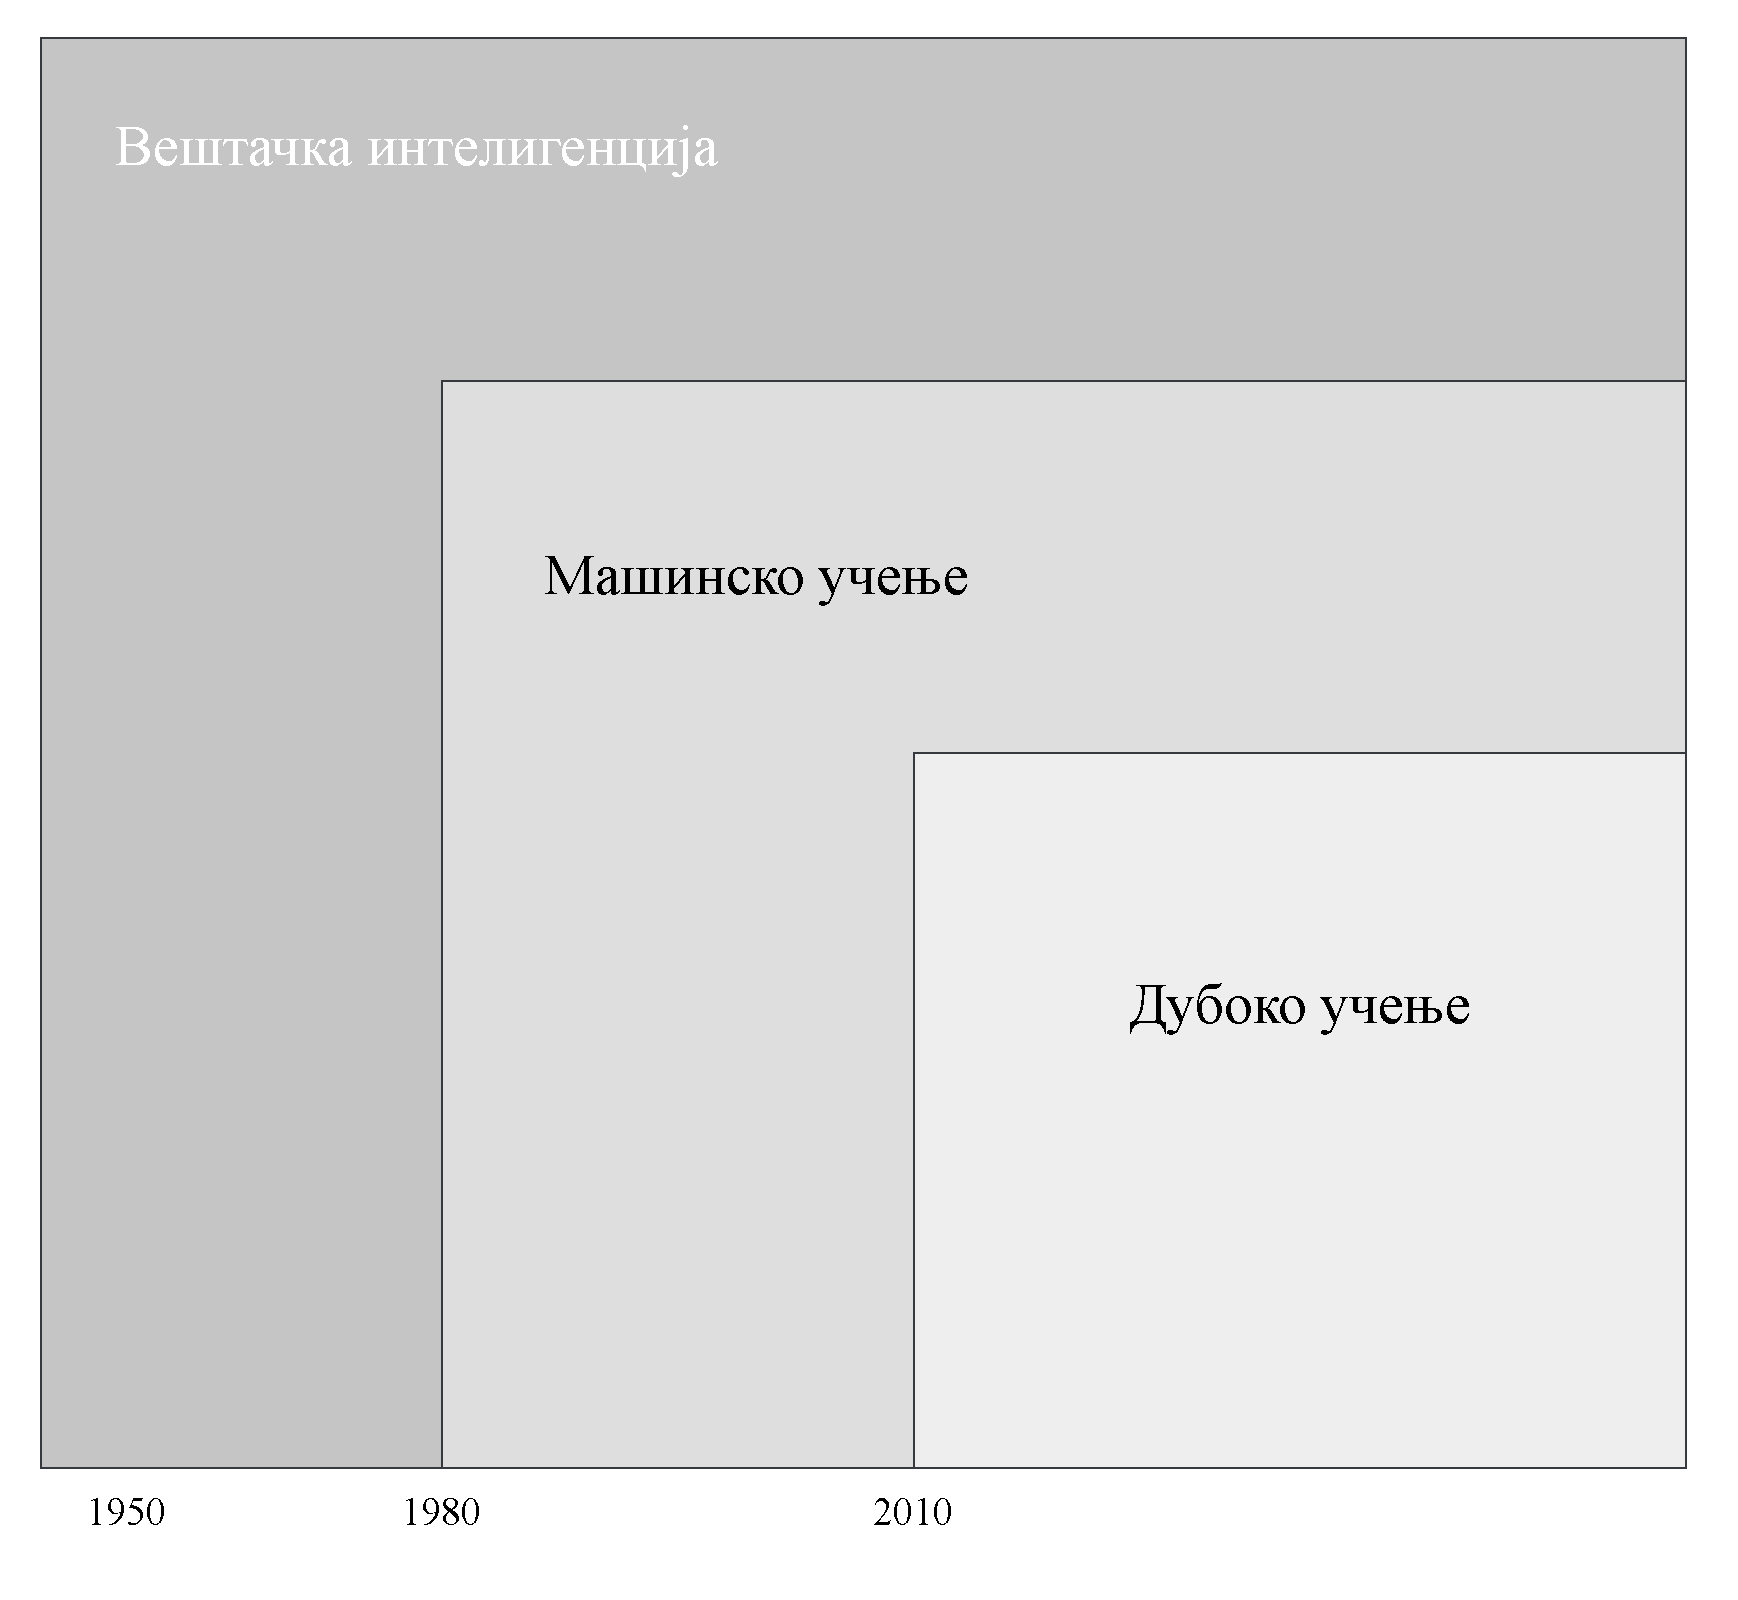
\includegraphics[width=\linewidth]{slike/финал.drawio.pdf}
    \caption{Веза између вештачке интелигенције, машинског и дубоког учења~\cite{Huawei2023AI}.}
    \label{fig:relationship}
\end{figure}

\vspace{1em}

Вештачка интелигенција може да се подели на јаку вештачку интелигенцију и слабу вештачку интелигенцију.

Јака вештачка интелигенција везана је за могућност стварања интелигнетних машина које могу да обављају задатке који захтевају логичко закључивање и решавање проблема. Верује се да машине ове врсте имају свест и самосвест и да могу да размишљају независно и дају најбоља решења за проблеме. Јака вештачка интелигенција, такође има себи својствене вредности и поглед на свет, поседује и инстикте, као што су потребе за преживљавањем и сигурношћу, баш као и сва жива бића. 

Слаба вештачка интелигенција описује околности онда када није способна да направи машине које заиста могу да расуђују и решавају проблеме. Ове машине могу да делују паметно, али заправо немају интелгенцију или самосвест.  

Дубоко учење односи се на тренирање дубоких неуронских мрежа. На примеру предвиђања цена кућа у зависности од њихове величине биће објашњено шта је једноставна неуронска мрежа, а у наставку ће бити разматране и дубоке неуронске мреже. 

Скуп података се састоји од шест кућа. Познати подаци су квадратура сваке куће и одговарајућа цена, а потребно је одредити функцију за предвиђање цене куће. Цене никада не могу бити негативне. Плава линија на слици~\ref{fig:предвиђањеценакућа} представља функцију за предвиђање цене куће као функције њене величине. Поменута функција представљена плавом линијом може да се посматра као веома једноставна неуронска мрежа~\cite{cs230notes}.

\begin{figure}[H]
    \centering
    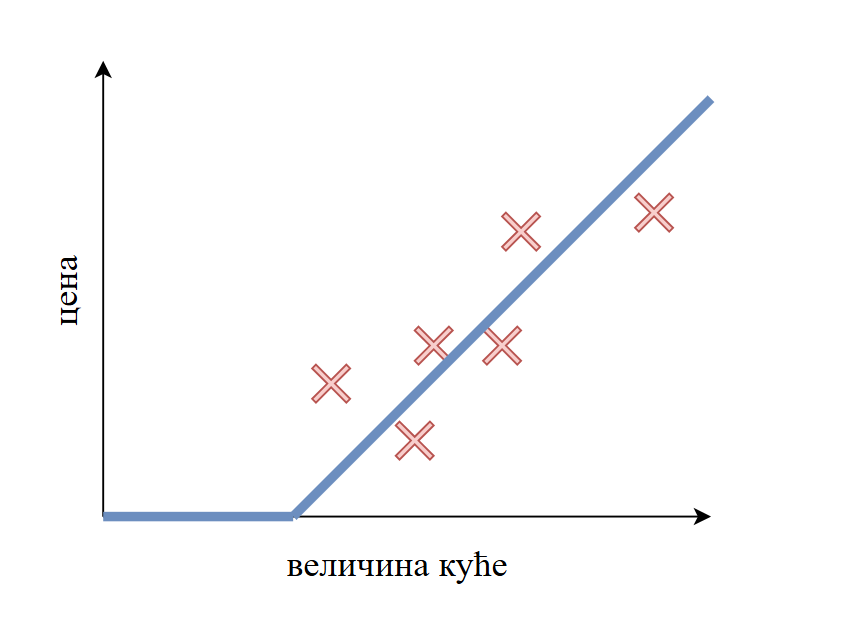
\includegraphics[width=\linewidth]{slike/куће.png}
    \caption{Предвиђање цена кућа.}
    \label{fig:предвиђањеценакућа}
\end{figure}

Мала једноставна неуронска мрежа коју чини један неурон приказана је на слици~\ref{fig:jednostavnaneuronskamreza}. Улаз у неуронску мрежу је променљива x која представља величину куће. Променљива $x$ улази у круг, односно у један неурон у неуронској мрежи. Излаз из неурона је цена означена променљивом $y$. Неурон имплементира функцију означену плавом бојом на слици~\ref{fig:предвиђањеценакућа} тако што прво прихвата величину куће као улазни податак, затим рачуна линеарну функцију, узима максимум од нуле и од вредности улаза и на излазу даје процену цене. Поменута функција означена плавом бојом коју имплементира неурон зове се ReLU (енгл. \textit{rectified linear unit}) функција. 

\begin{figure}[H]
    \centering
    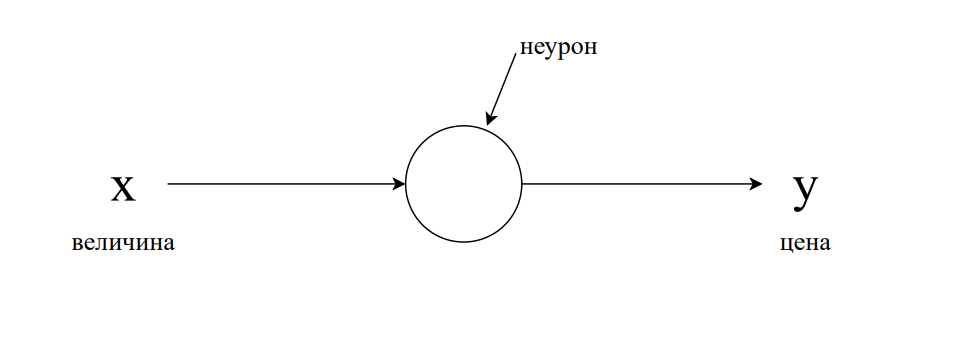
\includegraphics[width=\linewidth]{slike/neuron3png.png}
    \caption{Једноставна неуронска мрежа.}
    \label{fig:jednostavnaneuronskamreza}
\end{figure}

На слици~\ref{fig:slikaрелу} иста функција приказана је и у општем облику.

\begin{figure}[H]
    \centering
    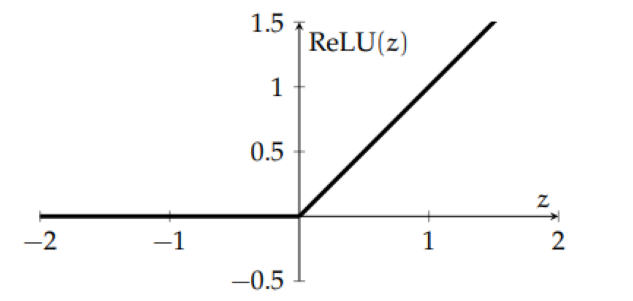
\includegraphics[width=\linewidth]{slike/РЕЛУ2.png}
    \caption{ReLU активациона функција~\cite{mit_intro_ml_lecture22}.}
    \label{fig:slikaрелу}
\end{figure}

Математички, ReLU активациона функција у општем облику дефинисана је као

\begin{equation}
\text{ReLU}(z)=
\left\{
\begin{array}{ll}
0 \quad \text{  за } z<0 \\[-4pt]
z \quad \text{ у супротном}
\end{array}
\right. = max(0,z)
\label{деф:релу}
\end{equation}

\vspace{1em}

Већа неуронска мрежа се прави груписањем и слагањем више појединачних неурона заједно и биће разматрана у наставку ослањајући се на претходни пример.

Цену куће, поред њене величине, одређују и друге карактеристике. На пример, број спаваћих соба и величина породице. Величина куће у квадратним метрима и број спаваћих соба одређују да ли кућа одговара величини породице. Поштански број куће, односно место где се налази кућа, говори колико је кућа удаљена од прехрамбене продавнице и школе и да ли до тамо може пешке да се стигне или је потребно ићи аутомобилом. Економски статус насеља је још једна карактеристика која одређује цену куће. Поштански број и економски статус насеља одређују квалитет школе у Сједињеним Америчким Државама, али и у неким другим земљама.

Сваки од кругова приказаних на слици~\ref{fig:slikaviseneurona} може да имплементира ReLU функцију активације или неку другу нелинеарну функцију, тако да на основу величине куће и броја спаваћих соба може да се процени величина породице која намерава да купи кућу, приступачност насеља за пешаке може да се процени на основу поштанског броја насеља, а квалитет школе на основу економског статуса и поштанског броја насеља. У овом примеру променљива $x$ представља сва четири улаза, а променљива $y$ представља цену куће коју је потребно предвидети. Груписањем поједниначних неурона приказаних на слици~\ref{fig:jednostavnaneuronskamreza} добија се већа неуронска мрежа приказана на слици~\ref{fig:slikaviseneurona}~\cite{cs230notes}.

\vspace{2em}

\begin{figure}[H]
    \centering
    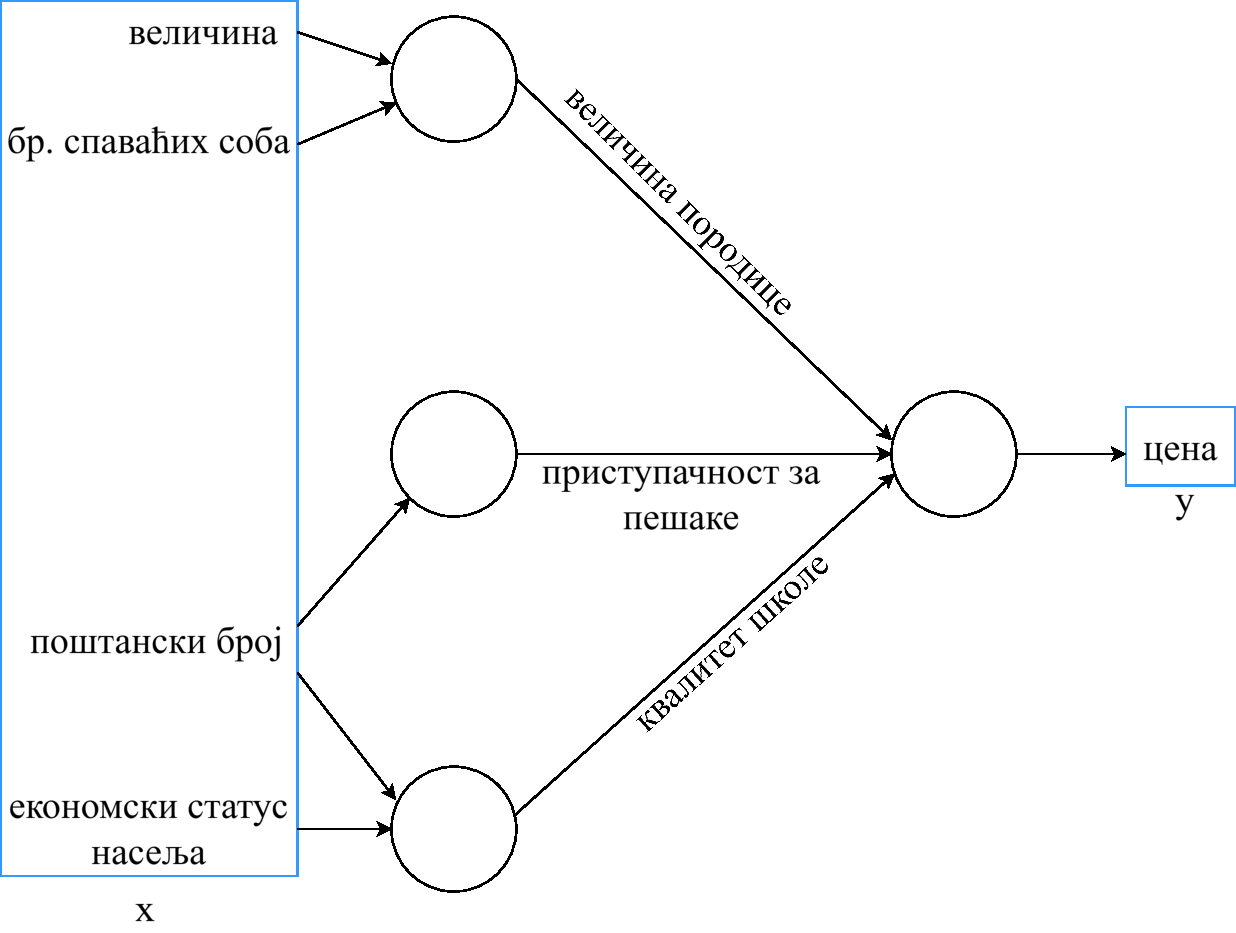
\includegraphics[width=\linewidth]{slike/sreca3.drawio.pdf}
    \caption{Неуронска мрежа са више неурона.}
    \label{fig:slikaviseneurona}
\end{figure}

Улаз у неуронску мрежу на слици~\ref{fig:slikaviseneurona} математички се означава као скуп улазних карактеристика $x_1$, $x_2$, $x_3$, $x_4$. Међупроменљиве које представљају величину породице, приступачност за пешаке и квалитет школе означене су са $a_1$, $a_2$, $a_3$ ($a_i$ међупроменљиве су скривене јединице или скривени неурони). Свака од $a_i$ међупроменљивих може да се представи као неуронска мрежа са једним неуроном и подскупом улазних променнљивих $x_1$, . . . , $x_4$. На основу наведеног изводе се следеће једначине:


\begin{equation}
a_1 = \text{ReLU}(\theta_1 x_1 + \theta_2 x_2 + \theta_3)
\end{equation}

\begin{equation}
\hspace{-1.3cm}a_2 = \text{ReLU}(\theta_4 x_3 + \theta_5)
\end{equation}

\begin{equation}
a_3 = \text{ReLU}(\theta_6 x_3 + \theta_7 x_4 + \theta_8)
\end{equation}

где су $(\theta_1, \dots, \theta_8)$ параметри. Сада се коначни излаз  
$\bar{h_\theta}(x)$ представља као линеарна функција са улазима $a_1$, $a_2$, $a_3$ и добија се једначина:

\begin{equation} \label{eq:5}
\bar{h_\theta}(x) = \theta_9 a_1 + \theta_{10} a_2 + \theta_{11} a_3 + \theta_{12}
\end{equation}

где $\theta$ садржи све параметре $(\theta_1, \dots, \theta_{12})$. 

Излаз је представљен комплексном функцијом у зависности од променљиве $x$ са параметрима $\theta$~\cite{NgMa2023CS229Notes}. 

\vspace{3em}








\subsection{Биолошке неуронске мреже}

Биолошке неуронске мреже биле су инспирација за стварање вештачких неуронских мрежа. Претходно поменуте скривене јединице $a_1, \dots, a_m$ одговарају неуронима у биолошкој неуронској мрежи, док параметри $\theta_i$ одговарају синапсама биолошке неуронске мреже. Ипак, није потпуно разјашњено колико су дубоке вештачке неуронске мреже сличне биолошким неуронским мрежама. У данашње време поједине вештачке неуронске мреже могу да имају 1000 слојева, док, са друге стране, вероватно мали број неуронаучника сматра да биолошке неуронске мреже могу имати толико слојева. Штавише, отворено је питање да ли људски мозак обнавља своје неуронске мреже на начин сличан ономе како научници из области рачунарства обучавају вештачке неуронске мреже (користећи \textit{backpropagation} методу). 

Људски мозак се састоји од великог броја међусобно повезаних неурона (нервних ћелија). Биолошки неурон чине три главна дела приказана на слици~\ref{fig:biologicalneuron}:

\begin{itemize}
  \item Дендрити
  \item Тело ћелије
  \item Аксон
\end{itemize}

Дендрити представљају продужетке тела ћелије и служе за прихватање сигнала од других неурона. Тело ћелије обрађује улазне сигнале, односно сабира сигнале са више улаза. Аксон је један дугачак продужетак који преноси сигнал од тела ћелије до других неурона, односно шаље обрађене сигнале ка другим неуронима. Тачка контакта између аксона једне ћелије и дендрита друге ћелије зове се синапса.    



\begin{figure}[H]
    \centering
    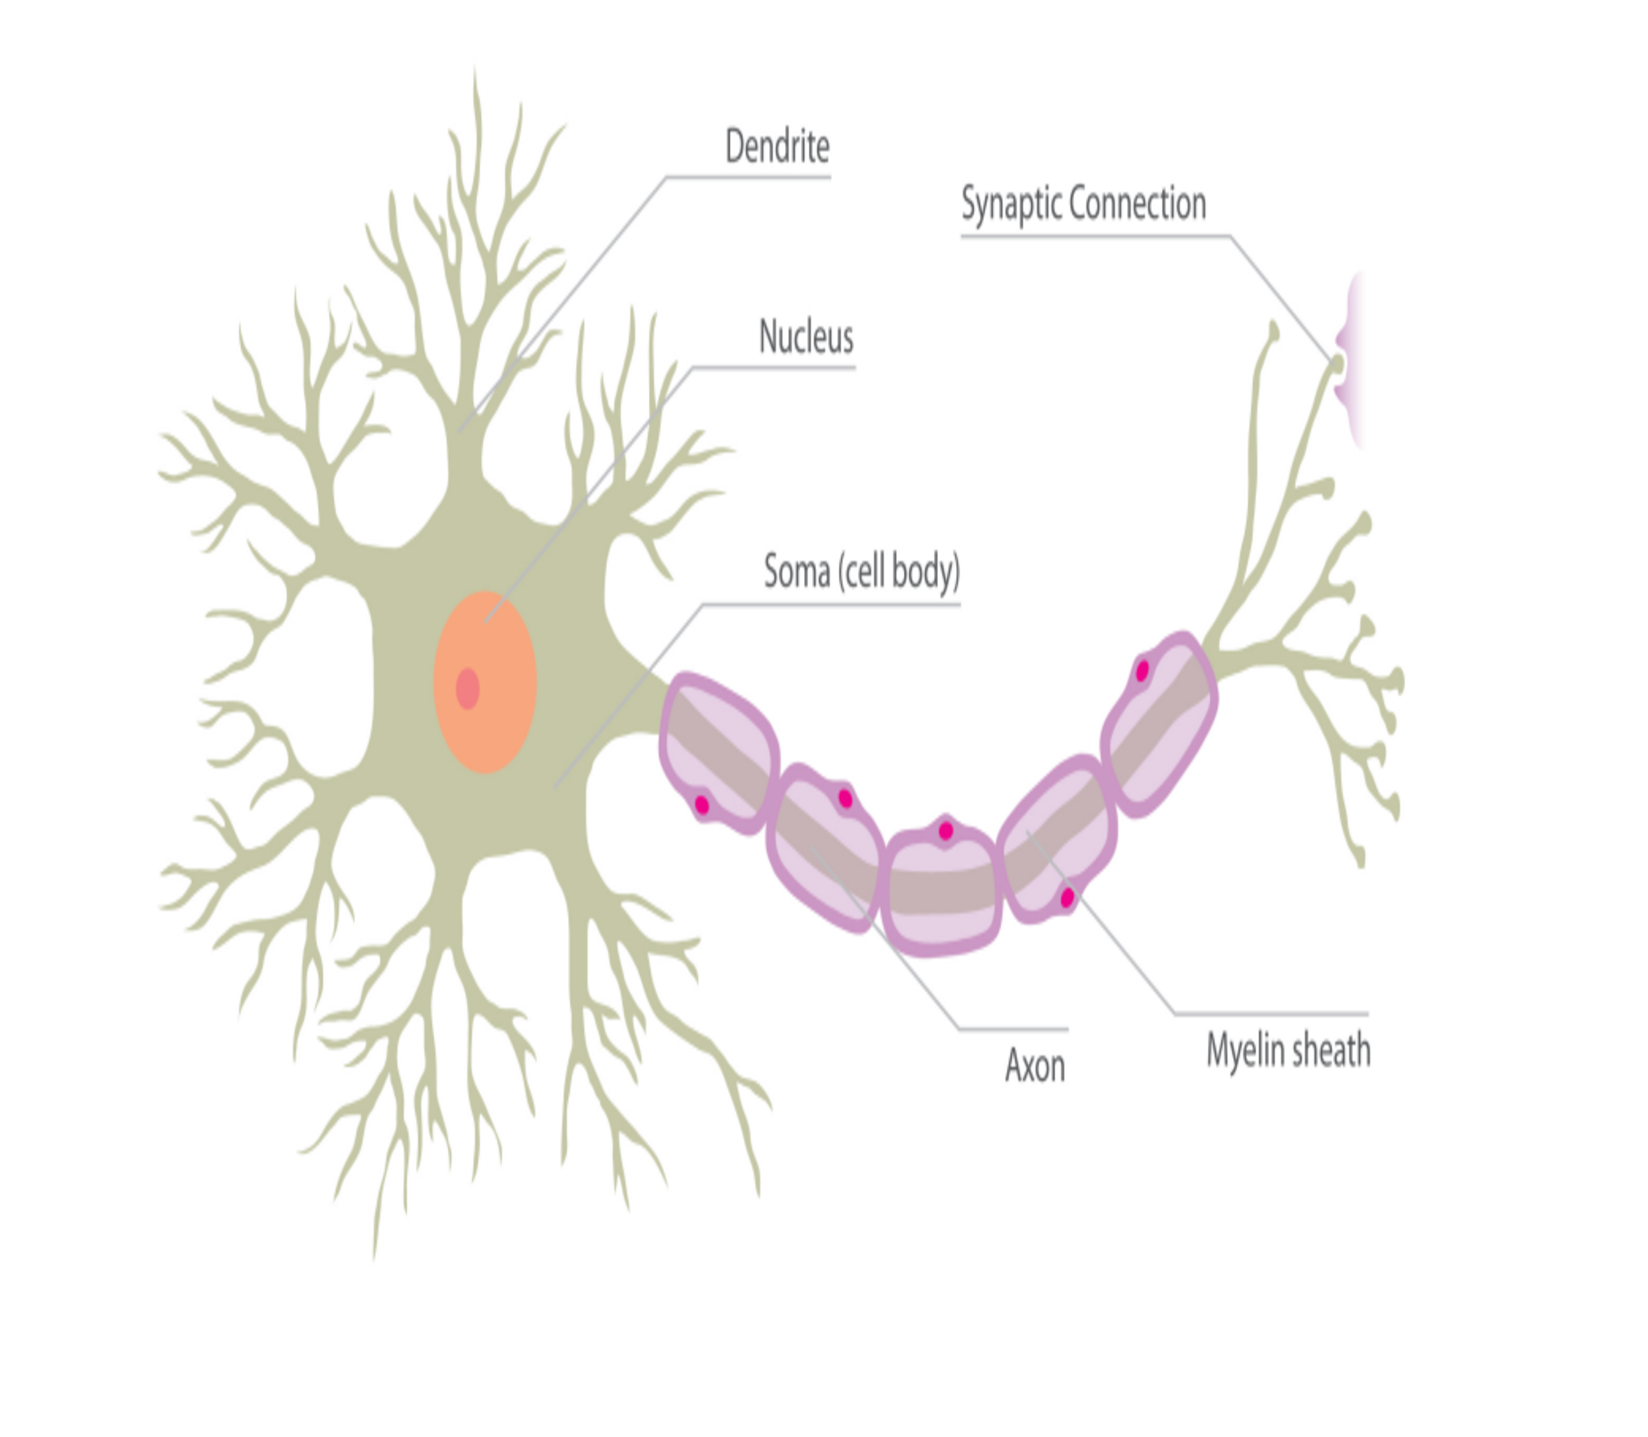
\includegraphics[width=\linewidth]{slike/bioNeuro7.pdf}
    \caption{Структура биолошког неурона~\cite{Fountas2011}.}
    \label{fig:biologicalneuron}
\end{figure}



\subsection{Потпуно повезане неуронске мреже}

Неуронска мрежа се заправо имплементира само задавањем улаза $x$ и излаза $y$ за одређени број примера у оквиру скупа за тренирање. Све остале карактеристике у средини (величина породице, приступачност за пешаке, квалитет школе) неуронска мрежа сама одређује.

 У облику у ком је треба имплементирати приказана је на слици~\ref{fig:имплементацјанмреже}. То је неуронска мрежа са четири улаза где улазне карактеристике могу бити величина куће, број спаваћих соба, поштански број насеља и економски статус насеља. Посао неуронске мреже је да на основу улазних карактеристика предвиди цену $y$. Кругови приказани на слици~\ref{fig:имплементацјанмреже} се још називају и скривене јединице, а улази сваког круга су све четири улазне карактеристике. На пример, уместо да први чвор представља величину породице и да величина породице зависи само од карактеристика $x_1$ и $x_2$ неуронска мрежа треба сама да одлучи шта ће тај чвор да представља на основу све четири дате улазне карактеристике.

 За слој уоквирен плавом бојом (улазни слој) и слој у средини који се састоји од три скривене јединице каже се да су густо повезани јер је свака улазна карактеристика повезана са сваким од кругова у средини. Важна особина неуронске мреже је њена спосоност да, уз довољну количину података $x$ и $y$, односно довољан број $(x, y)$  примера за тренирање, може да одреди функције које тачно пресликавају $x$ на $y$. Ово је основна структура неуронске мреже.

 \vspace{2em}
 \vspace{2em}

 
\begin{figure}[H]
    \centering
    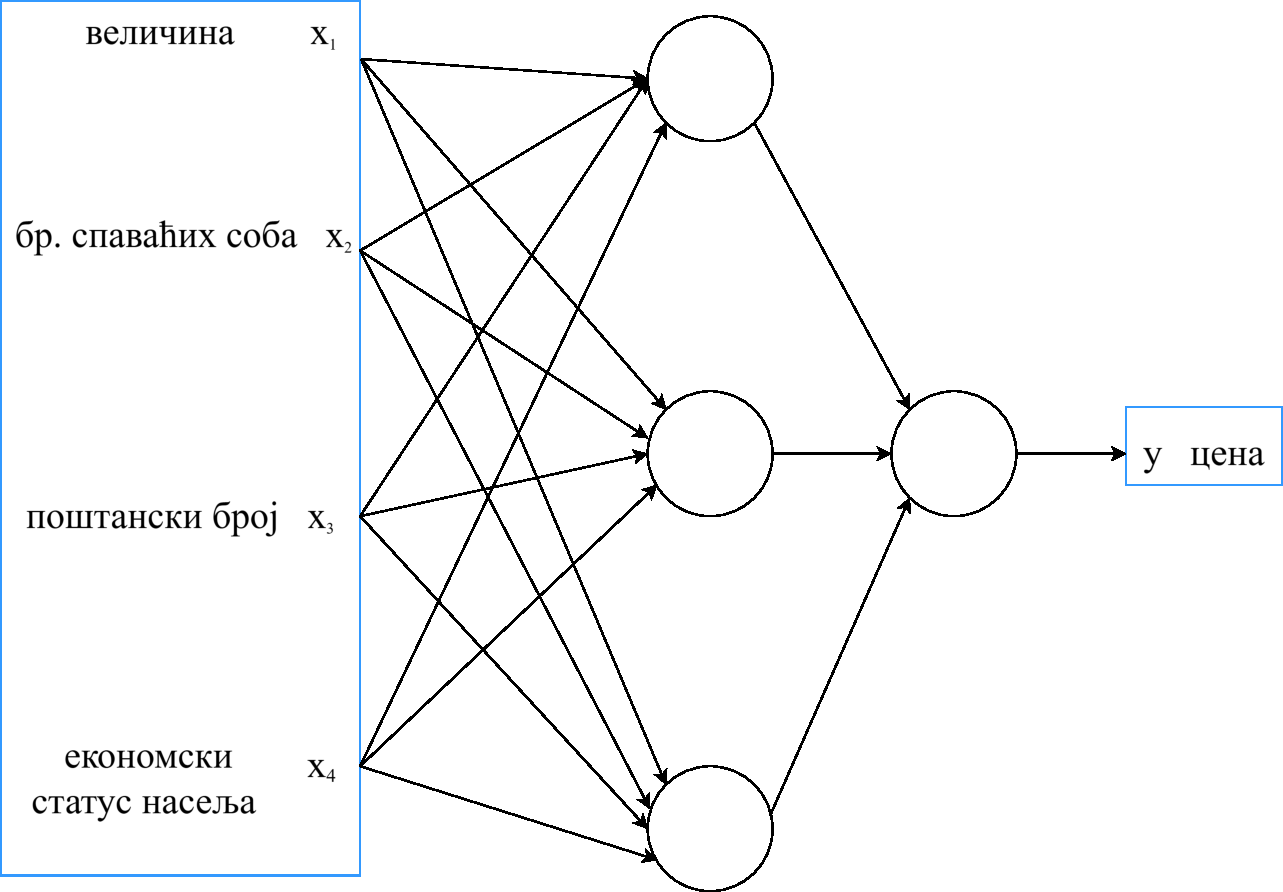
\includegraphics[width=\linewidth]{slike/nodes.drawio.pdf}
    \caption{Неуронска мрежа са више неурона - основна структура.}
    \label{fig:имплементацјанмреже}
\end{figure}

\vspace{2em}


У наставку ће ова мрежа бити дефинисана математички.

Неуронска мрежа описана једначином~\ref{eq:5} је направљена коришћењем претходног знања, тачније уверења о томе како су величина породице, приступачност за пешаке и квалитет школе одређени на основу улаза. Претпостављено је да је величина породице важна карактеристика коју треба разматрати и да може да се одреди само на основу величине куће и броја спаваћих соба. Такво претходно знање није увек доступно, тј. не зна се који улаз утиче на шта у неуронској мрежи. Стога је погодније увести параметре и на тај начин омогућити мрежи да сама учи из података. Једноставан начин за то јесте дефинисање међупроменљиве $a_1$ као функције у зависности од променљивих $x_1, \dots , x_4$ (међупроменљива $a_1$ зависи од свих улазних променљивих, а не само од $x_1$ и $x_2$):

\vspace{2em}

\begin{equation}
a_1 = \text{ReLU}(\omega_1^T x + b_1), \text{ где } \omega_1 \in \mathbb{R}^4 \text{ и } b_1 \in \mathbb{R}
\end{equation}

\begin{equation}
a_2 = \text{ReLU}(\omega_2^T x + b_2), \text{ где } \omega_2 \in \mathbb{R}^4 \text{ и } b_2 \in \mathbb{R}
\end{equation}

\begin{equation}
a_3 = \text{ReLU}(\omega_3^T x + b_3), \text{ где } \omega_3 \in \mathbb{R}^4 \text{ и } b_3 \in \mathbb{R}
\end{equation}

\vspace{2em}

Излаз $\bar{h_\theta}(x)$ се још увек дефинише коришћењем једначине (~\ref{eq:5}),а међупроменљиве $a_1$, $a_2$ и $a_3$ дефинисане су изнад. Оваква неуронска мрежа се зове \textbf{потпуно повезана неуронска мрежа} (енгл. \textit{fully connected neural network}) зато што све међупроменљиве $a_i$ зависе од свих улаза $x_i$~\cite{NgMa2023CS229Notes}. 
   
Још уопштеније, двослојна потпуно повезана неуронска мрежа са $m$ скривених јединица и $d$ димензионалним улазом $x \in \mathbb{R}^d$ дефинише се као


\begin{align}
\forall j \in [1, \dots, m], \quad  z_j &= \omega_j^{[1]^T}x + b_j^{[1]} \text{  где } \omega_j^{[1]} \in \mathbb{R}^d, b_j^{[1]} \in \mathbb{R} \\   
a_j &= \text{ReLU}(z_j), \notag \\
a &= {[a_1, \dots, a_m]}^T \in \mathbb{R}^m \notag \\
\bar{h_\theta}(x) &= \omega^{[2]^T}a + b^{[2]} \text{  где } \omega^{[2]} \in \mathbb{R}^m, b^{[2]} \in \mathbb{R}
\end{align}

Вектори у $\mathbb{R}^d$ се посматрају као вектори колона, конкретно $a$ је вектор колона са компонентама $a_1, a_2 \dots, a_m$. Индекси $^{[1]}$ и $^{[2]}$ су коришћени да би се разликовала два скупа параметара: $\omega_j^{[1]}$ (од којих је сваки вектор у $\mathbb{R}^d$) и $\omega^{[2]}$ (ово је вектор у $\mathbb{R}^m$).  


\vspace{2em}

\subsection{Дубоке потпуно повезане неуронске мреже}

На сликама~\ref{fig:logistic:regression},~\ref{fig:onehlayer},~\ref{fig:twohlayer} и~\ref{fig:fivehlayer} у наставку приказана је логистичка регресија, затим неуронска мрежа са једним скривеним слојем, неуронска мрежа са два скривена слоја и неуронска мрежа са пет скривених слојева, респективно. 

Логистичка регресија се сматра плитким моделом односно представља плитку неуронску мрежу и има само један слој. Супротно томе, модел на слици~\ref{fig:fivehlayer} представља дубоку неуронску мрежу. На слици~\ref{fig:onehlayer} приказана је неуронска мрежа са два слоја јер се улазни слој не рачуна, а укупан број слојева неуронске мреже чине скривени слојеви и излазни слој. Ова мрежа је такође плитка, али не толико као логистичка регресија.

\vspace{6em}

\begin{figure}[htpb]
    \centering
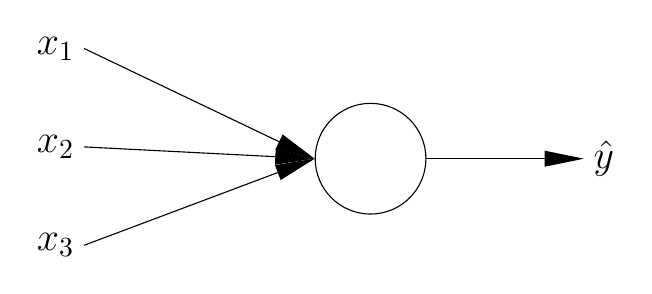
\begin{tikzpicture}[
    neuron/.style={circle, draw, minimum size=40pt, inner sep=0pt},
    input/.style={},
    >=stealth
]

% --- Input labels ---
\node (x1) at (-1,0.9) {\Large $x_1$};
\node (x2) at (-1,-0.35) {\Large $x_2$};
\node (x3) at (-1,-1.6) {\Large $x_3$};



% --- Output layer (1 neuron) ---
\node[neuron] (out) at (3,-0.5) {};

% --- Fully connect input to first hidden ---
\foreach \i in {1,2,3}
{
    \draw[-{Triangle[length=5mm, width=2mm]}] (x\i.east) -- (out.west);
    
}



% --- Output arrow and label ---
\draw[-{Triangle[length=5mm, width=2mm]}] (out.east) -- ++(2,0) node[right] {\Large $\hat{y}$};

\end{tikzpicture}
\vspace{20pt}
\caption{Логистичка регресија~\cite{cs230notes}.}
    \label{fig:logistic:regression}
\end{figure}

\setlength{\floatsep}{50pt}

\begin{figure}[htpb]
    \centering
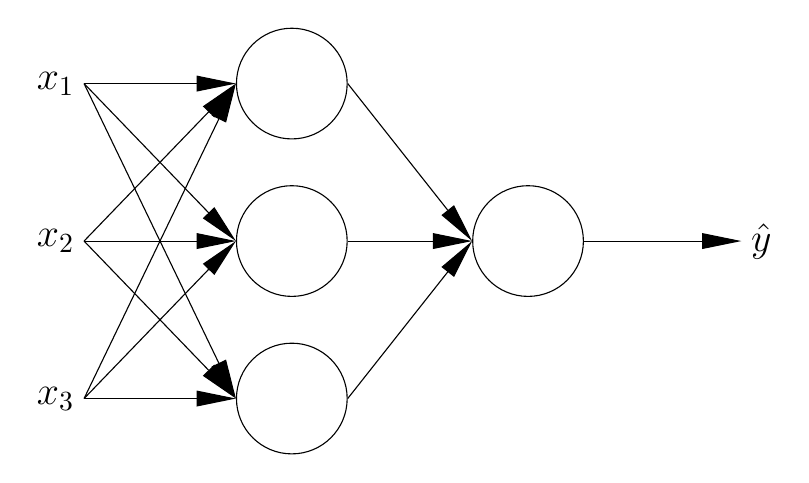
\begin{tikzpicture}[
    neuron/.style={circle, draw, minimum size=40pt, inner sep=0pt},
    input/.style={},
    >=stealth
]

% --- Input labels ---
\node (x1) at (1,0.5) {\Large $x_1$};
\node (x2) at (1,-1.5) {\Large $x_2$};
\node (x3) at (1,-3.5) {\Large $x_3$};

% --- First hidden layer (4 neurons) ---
\foreach \i in {1,...,3}
    \node[neuron] (h1\i) at (4,{2.5 - \i*2}) {};

% --- Output layer (1 neuron) ---
\node[neuron] (out) at (7,-1.5) {};

% --- Fully connect input to first hidden ---
\foreach \i in {1,2,3}
{
    \foreach \j in {1,...,3}
    {
        \draw[-{Triangle[length=5mm, width=2mm]}] (x\i.east) -- (h1\j.west);
    }
}

% --- Connect second hidden to output ---
\foreach \i in {1,...,3}
{
    \draw[-{Triangle[length=5mm, width=2mm]}] (h1\i.east) -- (out.west);
}

% --- Output arrow and label ---
\draw[-{Triangle[length=5mm, width=2mm]}] (out.east) -- ++(2,0) node[right] {\Large $\hat{y}$};

\end{tikzpicture}
\vspace{20pt}
\caption{Неуронска мрежа са једним скривеним слојем~\cite{cs230notes}.}
    \label{fig:onehlayer}
\end{figure}


\begin{figure}[htpb]
    \centering
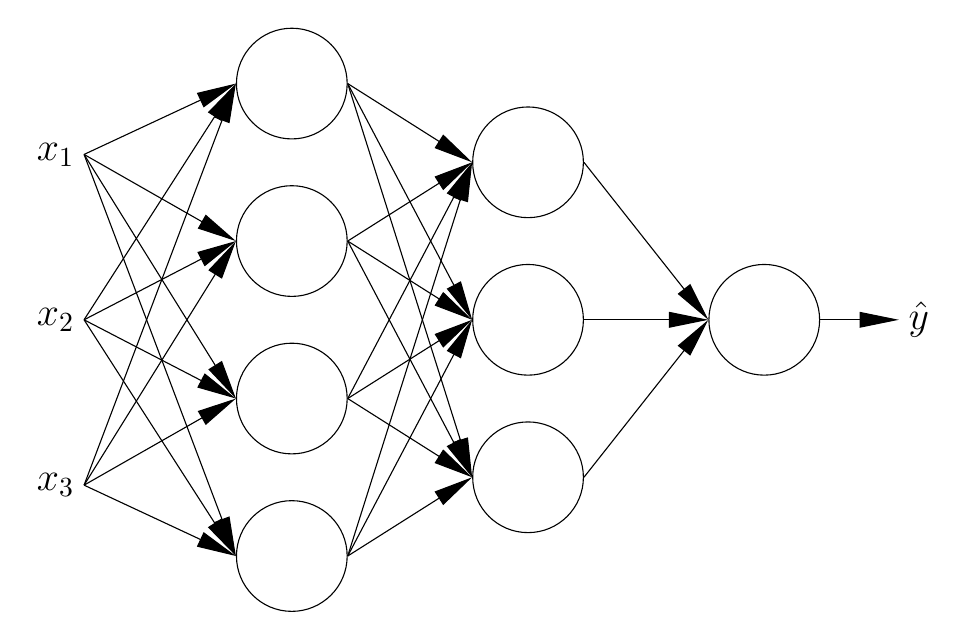
\begin{tikzpicture}[
    neuron/.style={circle, draw, minimum size=40pt, inner sep=0pt},
    input/.style={},
    >=stealth
]

% --- Input labels ---
\node (x1) at (-1,-0.4) {\Large $x_1$};
\node (x2) at (-1,-2.5) {\Large $x_2$};
\node (x3) at (-1,-4.6) {\Large $x_3$};

% --- First hidden layer (4 neurons) ---
\foreach \i in {1,...,4}
    \node[neuron] (h1\i) at (2,{2.5 - \i*2}) {};

% --- Second hidden layer (3 neurons) ---
\foreach \i in {1,...,3}
    \node[neuron] (h2\i) at (5,{1.5 - \i*2}) {};

% --- Output layer (1 neuron) ---
\node[neuron] (out) at (8,-2.5) {};

% --- Fully connect input to first hidden ---
\foreach \i in {1,2,3}
{
    \foreach \j in {1,...,4}
    {
        \draw[-{Triangle[length=5mm, width=2mm]}] (x\i.east) -- (h1\j.west);
    }
}

% --- Fully connect first hidden to second hidden ---
\foreach \i in {1,...,4}
{
    \foreach \j in {1,...,3}
    {
        \draw[-{Triangle[length=5mm, width=2mm]}] (h1\i.east) -- (h2\j.west);
    }
}

% --- Connect second hidden to output ---
\foreach \i in {1,...,3}
{
    \draw[-{Triangle[length=5mm, width=2mm]}] (h2\i.east) -- (out.west);
}

% --- Output arrow and label ---
\draw[-{Triangle[length=5mm, width=2mm]}] (out.east) -- ++(1,0) node[right] {\Large $\hat{y}$};

\end{tikzpicture}
\caption{Неуронска мрежа са два скривена слоја~\cite{cs230notes}.}
    \label{fig:twohlayer}
\end{figure}





\begin{figure}[!ht]
    \centering
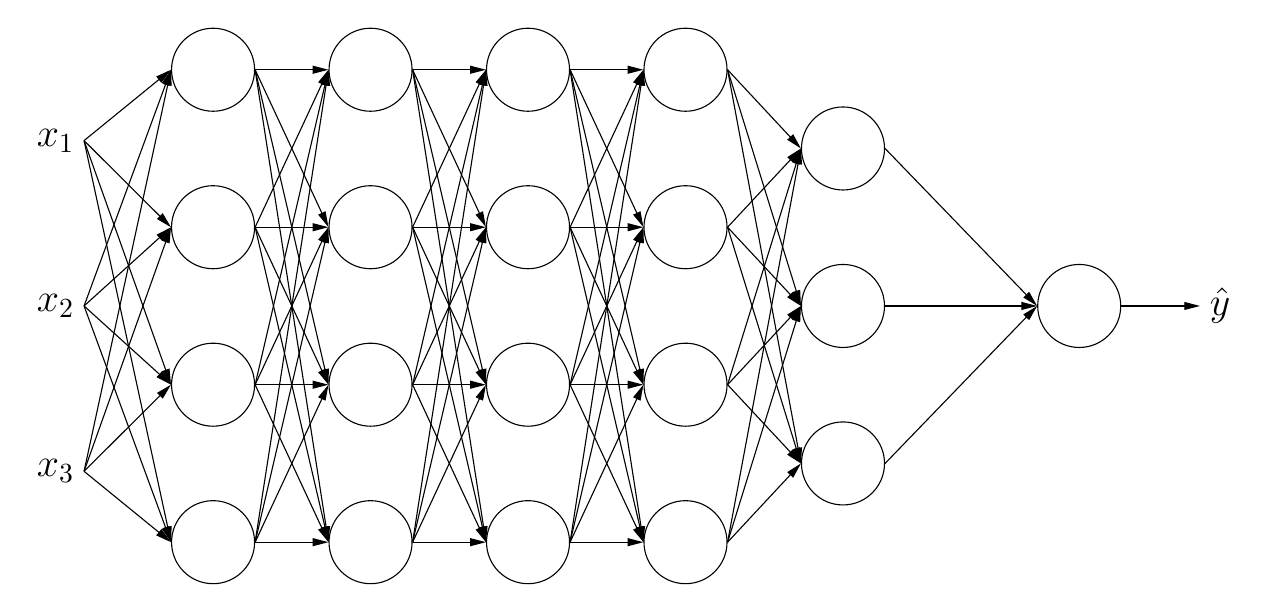
\begin{tikzpicture}[
    neuron/.style={circle, draw, minimum size=30pt, inner sep=0pt},
    input/.style={},
    >=stealth
]

% --- Input labels ---
\node (x1) at (-9,-0.4) {\Large $x_1$};
\node (x2) at (-9,-2.5) {\Large $x_2$};
\node (x3) at (-9,-4.6) {\Large $x_3$};

% --- First hidden layer (4 neurons) ---
\foreach \i in {1,...,4}
    \node[neuron] (h1\i) at (-7,{2.5 - \i*2}) {};

% --- second hidden layer (4 neurons) ---
\foreach \i in {1,...,4}
    \node[neuron] (h2\i) at (-5,{2.5 - \i*2}) {};

% --- Third hidden layer (4 neurons) ---
\foreach \i in {1,...,4}
    \node[neuron] (h3\i) at (-3,{2.5 - \i*2}) {};

% --- Fourth hidden layer (4 neurons) ---
\foreach \i in {1,...,4}
    \node[neuron] (h4\i) at (-1,{2.5 - \i*2}) {};

% --- Fifth hidden layer (3 neurons) ---
\foreach \i in {1,...,3}
    \node[neuron] (h5\i) at (1,{1.5 - \i*2}) {};

% --- Output layer (1 neuron) ---
\node[neuron] (out) at (4,-2.5) {};

% --- Fully connect input to first hidden ---
\foreach \i in {1,2,3}
{
    \foreach \j in {1,...,4}
    {
        \draw[-{Triangle[length=2mm, width=1mm]}] (x\i.east) -- (h1\j.west);
    }
}

% --- Fully connect first hidden to second hidden ---
\foreach \i in {1,...,4}
{
    \foreach \j in {1,...,4}
    {
        \draw[-{Triangle[length=2mm, width=1mm]}] (h1\i.east) -- (h2\j.west);
    }
}

% --- Fully connect second hidden to third hidden ---
\foreach \i in {1,...,4}
{
    \foreach \j in {1,...,4}
    {
        \draw[-{Triangle[length=2mm, width=1mm]}] (h2\i.east) -- (h3\j.west);
    }
}

% --- Fully connect third hidden to fourth hidden ---
\foreach \i in {1,...,4}
{
    \foreach \j in {1,...,4}
    {
        \draw[-{Triangle[length=2mm, width=1mm]}] (h3\i.east) -- (h4\j.west);
    }
}

% --- Fully connect fourth hidden to fifth hidden ---
\foreach \i in {1,...,4}
{
    \foreach \j in {1,...,3}
    {
        \draw[-{Triangle[length=2mm, width=1mm]}] (h4\i.east) -- (h5\j.west);
    }
}

% --- Connect fifth hidden to output ---
\foreach \i in {1,...,3}
{
    \draw[-{Triangle[length=2mm, width=1mm]}] (h5\i.east) -- (out.west);
}

% --- Output arrow and label ---
\draw[-{Triangle[length=2mm, width=1mm]}] (out.east) -- ++(1,0) node[right] {\Large $\hat{y}$};

\end{tikzpicture}
\caption{Неуронска мрежа са пет скривених слојева~\cite{cs230notes}.}
    \label{fig:fivehlayer}
\end{figure}


На слици~\ref{fig:dnn} приказана је дубока неуронска мрежа са четири слоја од којих су три слоја скривени слојеви. У првом и другом скривеном слоју је по пет јединица, а у трећем скривеном слоју су три јединице. У наставку ће број чворова у различитим слојевима неуронске мреже бити дефинисан математички.

\begin{figure}[!ht]
    \centering
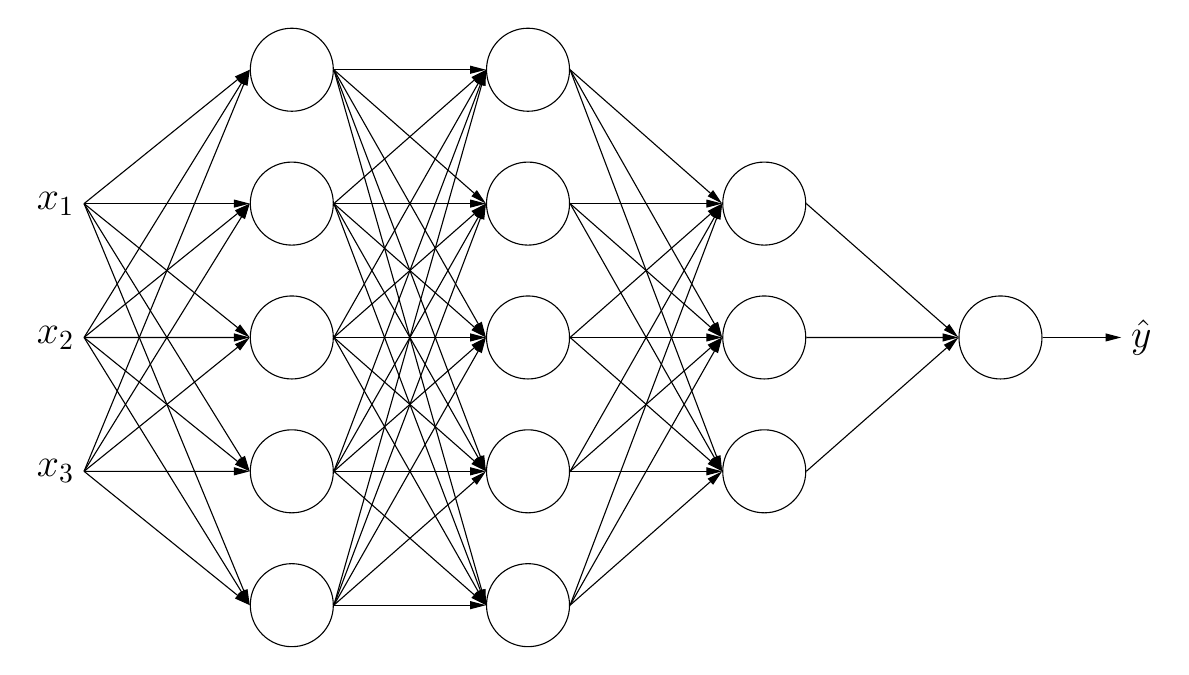
\begin{tikzpicture}[
    neuron/.style={circle, draw, minimum size=30pt, inner sep=0pt},
    input/.style={},
    >=stealth
]

% --- Input labels ---
\node (x1) at (-8,-0.9) {\Large $x_1$};
\node (x2) at (-8,-2.6) {\Large $x_2$};
\node (x3) at (-8,-4.3) {\Large $x_3$};

% --- First hidden layer (4 neurons) ---
\foreach \i in {1,...,5}
    \node[neuron] (h1\i) at (-5,{2.5 - \i*1.7}) {};

% --- Second hidden layer (4 neurons) ---
\foreach \i in {1,...,5}
    \node[neuron] (h2\i) at (-2,{2.5 - \i*1.7}) {};

% --- Third hidden layer (3 neurons) ---
\foreach \i in {1,...,3}
    \node[neuron] (h3\i) at (1,{0.8 - \i*1.7}) {};

% --- Output layer (1 neuron) ---
\node[neuron] (out) at (4,-2.6) {};

% --- Fully connect input to first hidden ---
\foreach \i in {1,2,3}
{
    \foreach \j in {1,...,5}
    {
        \draw[-{Triangle[length=2mm, width=1mm]}] (x\i.east) -- (h1\j.west);
    }
}

% --- Fully connect first hidden to second hidden ---
\foreach \i in {1,...,5}
{
    \foreach \j in {1,...,5}
    {
        \draw[-{Triangle[length=2mm, width=1mm]}] (h1\i.east) -- (h2\j.west);
    }
}



% --- Fully connect second hidden to third hidden ---
\foreach \i in {1,...,5}
{
    \foreach \j in {1,...,3}
    {
        \draw[-{Triangle[length=2mm, width=1mm]}] (h2\i.east) -- (h3\j.west);
    }
}


% --- Connect third hidden to output ---
\foreach \i in {1,...,3}
{
    \draw[-{Triangle[length=2mm, width=1mm]}] (h3\i.east) -- (out.west);
}

% --- Output arrow and label ---
\draw[-{Triangle[length=2mm, width=1mm]}] (out.east) -- ++(1,0) node[right] {\Large $\hat{y}$};

\end{tikzpicture}
\caption{Дубока неуронска мрежа~\cite{cs230notes}.}
    \label{fig:dnn}
\end{figure}


Укупан број слојева у неуронској мрежи означава се са $L$.

\begin{equation}
L = 4
\end{equation}

Број јединица или чворова у слоју $l$ означен је са $n^{[l]}$ ($n$ са горњим индексом $l$). 

Улаз може да се означи као слој 0, први скривени слој као слој 1, други скривени слој као слој 2, трећи скривени слој као слој 3 и излазни слој као слој 4. Стога, број чворова у слоју 1 математички може да се запише као

\begin{equation}
n^{[1]} = 5
\end{equation}

јер се у слоју 1 налази пет скривених јединица. 
За остале слојеве важи 

\begin{equation}
n^{[2]} = 5,\quad n^{[3]} = 3, \quad n^{[4]} = n^{[L]} = 1
\end{equation}

За улазни слој важи

\begin{equation}
n^{[0]} = n_x = 3
\end{equation}


За сваки слој $l$ активације се означавају са $a^{[l]}$. Током процеса ширења унапред (енгл. \textit{forward propagation}) добија се да је

\begin{equation}
a^{[l]} = g^{[l]}(z^{[l]})
\end{equation}

Тежине за израчунавање вредности $z^{[l]}$ у слоју $l$ означавају се са $w^{[l]}$. Слично томе, $b^{[l]}$ се користи за израчунавање вредности $z^{[l]}$. Улазне карактеристике су такође и активације слоја 0 и се означавају са $x$, па важи

\begin{equation}
x = a^{[0]}
\label{eq:equality}
\end{equation}

Активација последњег слоја једнака је предвиђеном излазу неуронске мреже.

\begin{equation}
a^{[L]} = \hat{y}
\end{equation}

\subsubsection{Процес ширења унапред у дубокој неуронској мрежи}

Неуронска мрежа ширења унапред (енгл. \textit{feedforward neural network}) је вештачка неуронска мрежа код које се подаци крећу само у једном смеру - од улаза ка излазу. Код такве мреже улаз у неурон никада не може да зависи од излаза из тог неурона~\cite{mit_intro_ml_lecture22}.

Прво ће бити објашњен процес ширења унапред за један пример за тренирање, $x$. Касније ће исти процес бити објашњен са векторима, односно изводиће се истовремено на целом скупу података за тренирање. 

Ако је дат један примерак за тренирање $x$, онда се активације првог слоја рачунају на начин описан у наставку. За први слој важи да је улаз слоја 1, $z^{[1]}$ једнак

\begin{equation}
x:\quad z^{[1]} = w^{[1]}x + b^{[1]}
\label{eq:activation_layer1}
\end{equation}

где су $w^{[1]}$ и  $b^{[1]}$ параметри који  утичу на активације у слоју 1. Активациона функција je означена са $g$ и ако се посматра први слој неуронске мреже онда се у горњем индексу функције $g$ додаје јединица. Активације слоја 1 се израчунавају помоћу једначине~\ref{eq:activation}, односно применом активационе функције на $z^{[1]}$.  

\begin{equation}
a^{[1]} = g^{[1]}(z^{[1]})
\label{eq:activation}
\end{equation}

За слој 2 важи једначина~\ref{eq:слој2}

\begin{equation}
z^{[2]} = w^{[2]}a^{[1]} + b^{[2]}
\label{eq:слој2}
\end{equation}

где је $w^{[2]}$ матрица тежине, $a^{[1]}$ излаз из првог слоја односно активација претходног слоја - слоја 1, а $b^{[2]}$ бајас вектор за слој 2. Онда се активација слоја 2 израчунава као 

\begin{equation}
a^{[2]} = g^{[2]}(z^{[2]})
\end{equation}

Сличан запис користи се и за слој 3. За последњи слој - слој 4 важи

\begin{equation}
z^{[4]} = w^{[4]}a^{[3]} + b^{[4]}
\end{equation}

Излаз из неуронске мреже $\hat{y}$ се рачуна као

\begin{equation}
a^{[4]} = g^{[4]}(z^{[4]}) = \hat{y}
\end{equation}

Даље треба приметити да за $x$ из једначине~\ref{eq:activation_layer1} важи једнакост~\ref{eq:equality} тако да једначина~\ref{eq:activation_layer1} може да се напише и као

\begin{equation}
z^{[1]} = w^{[1]}a^{[0]} + b^{[1]}
\end{equation}

Једначине која описују поступак ширења унапред у општем случају су

\begin{equation}
z^{[l]} = w^{[l]}a^{[l-1]} + b^{[l]}, \quad a^{[l]} = g^{[l]}(z^{[l]})
\end{equation}

За поступак ширења унапред са векторима, за цели скуп података за тренирање једначине су сличне претходним једначинама, па за први слој важи

\begin{equation}
Z^{[1]} = w^{[1]}X + b^{[1]}
\label{eq:26}
\end{equation}

Уместо претходно поменутог једног примера $x$, сада су подаци за тренирање распоређени у различитим колонама. Како је $X=A^{[0]}$, једначина~\ref{eq:26} може да се запише и у следећем облику

\begin{equation}
Z^{[1]} = w^{[1]}A^{[0]} + b^{[1]} 
\label{eq:Z1}
\end{equation}

\begin{equation}
A^{[1]} = g^{[1]}(Z^{[1]})
\label{eq:A1}
\end{equation}

За следећи слој важи 

\begin{equation}
Z^{[2]} = w^{[2]}A^{[1]} + b^{[2]} 
\label{eq:Z2}
\end{equation}

\begin{equation}
A^{[2]} = g^{[2]}(Z^{[2]})
\label{eq:A2}
\end{equation}


Мала слова $z$ и $a$ у претходним изразима замењена су одговарајућим великим словима. Једначине које описују поступак ширења унапред у општем случају за векторе су

\begin{equation}
Z^{[l]} = W^{[l]}A^{[l-1]} + b^{[l]}, \quad A^{[l]} = g^{[l]}(Z^{[l]})
\end{equation}

На крају се добија предвиђање за све примере из скупа за тренирање и записује се као

\begin{equation}
\hat{Y} = g(Z^{[4]})=A^{[4]}
\label{eq:Y}
\end{equation}

За имплементацију поступка ширења унапред са векторима тј. са више примера на улазу потребно је користити \textit{for} петљу где је $l=1 \dots 4$, тачније где је $l=1 \dots L$. У петљи ће се израчунавати једначине~\ref{eq:Z1},~\ref{eq:A1},~\ref{eq:Z2},~\ref{eq:A2} и~\ref{eq:Y}, односно петља ће се користити за израчунавање активација за први, други, трећи и четврти слој приказан на слици~\ref{fig:dnn}.

\subsubsection{Димензије матрица}

За неуронску мрежу на следећој слици пише се да је $L=5$. Нерачунајући улазни слој неуронска мрежа има пет слојева, четири скривена или невидљива слоја и један излазни слој.



\begin{figure}[!ht]
    \centering
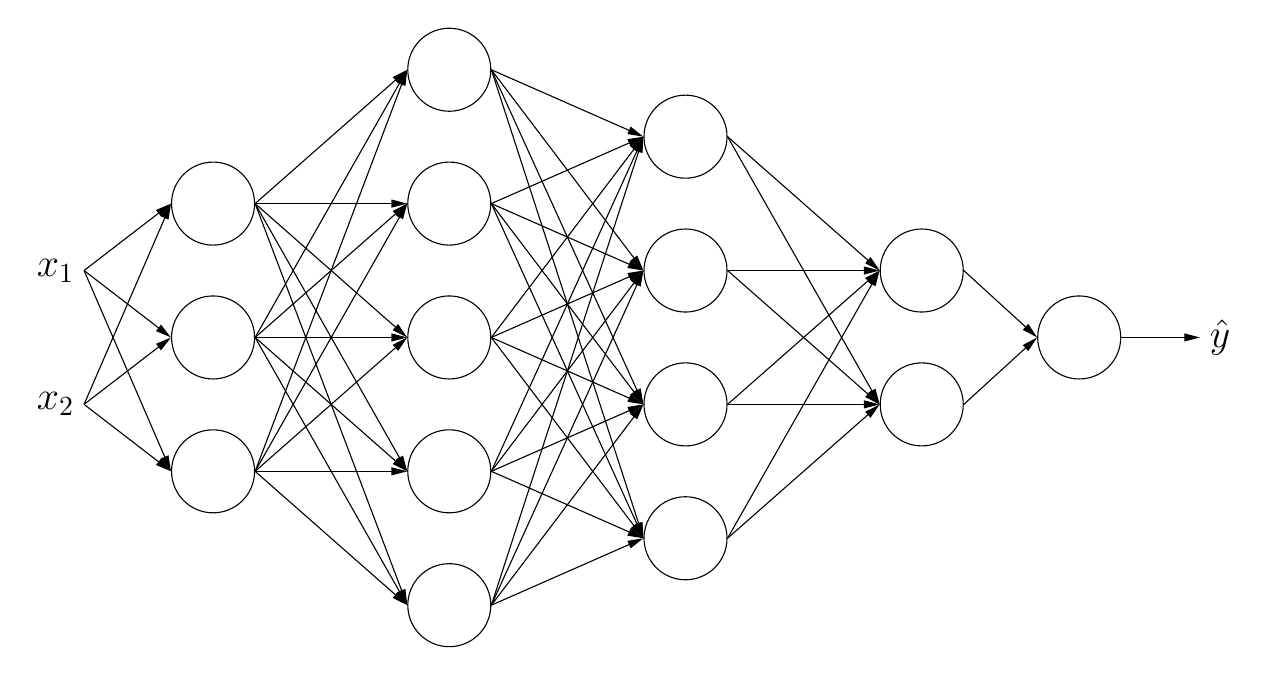
\begin{tikzpicture}[
    neuron/.style={circle, draw, minimum size=30pt, inner sep=0pt},
    input/.style={},
    >=stealth
]

% --- Input labels ---
\node (x1) at (-9,-1.75) {\Large $x_1$};
\node (x2) at (-9,-3.45) {\Large $x_2$};


% --- First hidden layer (4 neurons) ---
\foreach \i in {1,...,3}
    \node[neuron] (h1\i) at (-7,{0.8 - \i*1.7}) {};

% --- second hidden layer (4 neurons) ---
\foreach \i in {1,...,5}
    \node[neuron] (h2\i) at (-4,{2.5 - \i*1.7}) {};

% --- Third hidden layer (4 neurons) ---
\foreach \i in {1,...,4}
    \node[neuron] (h3\i) at (-1,{1.65 - \i*1.7}) {};

% --- Fourth hidden layer (4 neurons) ---
\foreach \i in {1,...,2}
    \node[neuron] (h4\i) at (2,{-0.05 - \i*1.7}) {};

% --- Output layer (1 neuron) ---
\node[neuron] (out) at (4,-2.6) {};

% --- Fully connect input to first hidden ---
\foreach \i in {1,2}
{
    \foreach \j in {1,...,3}
    {
        \draw[-{Triangle[length=2mm, width=1mm]}] (x\i.east) -- (h1\j.west);
    }
}

% --- Fully connect first hidden to second hidden ---
\foreach \i in {1,...,3}
{
    \foreach \j in {1,...,5}
    {
        \draw[-{Triangle[length=2mm, width=1mm]}] (h1\i.east) -- (h2\j.west);
    }
}

% --- Fully connect second hidden to third hidden ---
\foreach \i in {1,...,5}
{
    \foreach \j in {1,...,4}
    {
        \draw[-{Triangle[length=2mm, width=1mm]}] (h2\i.east) -- (h3\j.west);
    }
}

% --- Fully connect third hidden to fourth hidden ---
\foreach \i in {1,...,4}
{
    \foreach \j in {1,...,2}
    {
        \draw[-{Triangle[length=2mm, width=1mm]}] (h3\i.east) -- (h4\j.west);
    }
}

% --- Connect fifth hidden to output ---
\foreach \i in {1,...,2}
{
    \draw[-{Triangle[length=2mm, width=1mm]}] (h4\i.east) -- (out.west);
}

% --- Output arrow and label ---
\draw[-{Triangle[length=2mm, width=1mm]}] (out.east) -- ++(1,0) node[right] {\Large $\hat{y}$};

\end{tikzpicture}
\caption{Неуронска мрежа са пет слојева~\cite{cs230notes}.}
    \label{fig:fivelayers}
\end{figure}

Први корак имплементације процеса ширења унапред за неуронску мрежу са слике~\ref{fig:fivelayers} јесте дефинисање следеће једначине

\begin{equation}
z^{[1]} = w^{[1]}x + b^{[1]}
\label{eq:firststep}
\end{equation}

Први скривени слој има три скривене јединице па је

\begin{equation}
n^{[1]} = 3
\end{equation}

За остале слојеве важи 

\begin{equation}
n^{[2]} = 5,\quad n^{[3]} = 4, \quad n^{[4]} = 2, \quad n^{[5]} = 1
\end{equation}

док је за улазни слој

\begin{equation}
n^{[0]} = n_x = 2 
\end{equation}

\vspace{2em}

У наставку ће бити разматране димензије $z$, $w$ и $x$.

Вектор активација за први скривени слој је $z^{[1]}$ и његове димензије су (3, 1). Каже се и да је $z^{[1]}$ тродимензионални вектор, а у општем случају $z^{[1]}$ je $n^{[1]}$ - димензионални вектор или матрица димензија $(n^{[1]}, 1)$.

У овом случају дефинисане су две улазне карактеристике, па је $x$ димензија (2, 1), док је у општем случају $x$ димензија $(n^{[0]}, 1)$. Матрица $ w^{[1]}$ треба да буде таквих димензија да када се помножи са $(n^{[0]}, 1)$ вектором даје $(n^{[1]}, 1)$ вектор. У складу са правилима множења матрица, $ w^{[1]}$ у овом примеру мора бити матрица димензија (3, 2). Матрица димензија (3, 2) помножена са вектором димензија (2, 1) даје (3, 1) вектор. Множење матрица приказано је на слици~\ref{fig:матрица5}.   

\begin{figure}[H]
    \centering
    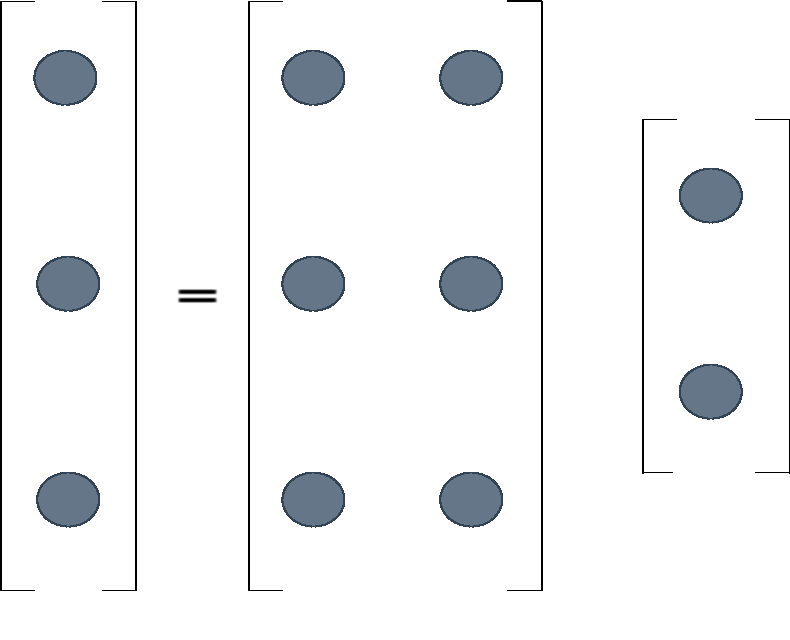
\includegraphics[width=0.8\linewidth]{slike/matricad4.drawio.pdf}
    \caption{Димензије матрице}
    \label{fig:матрица5}
\end{figure}

У општем случају $w^{[1]}$ мора бити матрица димензија $(n^{[1]}, n^{[0]})$.

\begin{equation}
w^{[1]} : \quad (n^{[1]}, n^{[0]})
\end{equation}

Димензије $w^{[2]}$ морају бити (5, 3) односно

\begin{equation}
w^{[2]} : \quad (n^{[2]}, n^{[1]})
\end{equation}

Код једначине~\ref{eq:zdva} димензије $z^{[2]}$, $w^{[2]}$ и $a^{[1]}$ су редом (5, 1), (5, 3), (3, 1).

\begin{equation}
z^{[2]} = w^{[2]}a^{[1]} + b^{[2]}
\label{eq:zdva}
\end{equation}

Слично, димензије параметра $w^{[3]}$ чине димензије следећег слоја тј. трећег слоја и димензије претходног слоја тј. другог слоја. 

\begin{equation}
w^{[3]} : \quad (4, 5)
\end{equation}

За остале слојеве важи

\begin{equation}
w^{[4]} : \quad (2, 4)
\end{equation}

\begin{equation}
w^{[5]} : \quad (1, 2)
\end{equation}

За слој $l$ у општем случају примењује се формула 
\begin{equation}
w^{[l]} : \quad (n^{[l]}, n^{[l-1]})
\end{equation}

Сада треба размотрити димензије вектора $b^{[1]}$ из једначине~\ref{eq:firststep}. Оне треба да одговарају димензијама $w^{[1]}x$. С обзиром на то да је производ $w^{[1]}x$ димензија (3, 1), треба му додати други вектор димензија (3, 1) да би се добио вектор димензија (3, 1) као резултат.

Слично претходном разматрању, код једначине~\ref{eq:zdva} димензије вектора $b^{[2]}$ треба да одговарају димензијама $w^{[2]}a^{[1]}$. С обзиром на то да је производ $w^{[2]}a^{[1]}$ димензија (5, 1), потребно је додати му други вектор димензија (5, 1) да би се добио вектор димензија (5, 1) као резултат. 

\vspace{2em}
У општем случају димензије параметра $b^{[1]}$ за први слој су   

\begin{equation}
b^{[1]} : \quad (n^{[1]}, 1)
\end{equation}

Димензије параметра $b^{[2]}$ за други слој у општем случају су 

\begin{equation}
b^{[2]} : \quad (n^{[2]}, 1)
\end{equation}

Стога, димензије параметра $b^{[l]}$ за слој $l$ су 

\begin{equation}
b^{[l]} : \quad (n^{[l]}, 1)
\end{equation}

\vspace{2em}

Како је $z^{[l]}=g^{[l]}(a^{[l]})$, онда $z^{[l]}$ и $a^{[l]}$ треба да буду истих димензија код ове врсте неуронских мрежа.

У наставку ће бити размотрена имплементација са векторима, за више примера. Димензије параметара $w^{[1]}$ и $b^{[1]}$ ће остати исте, али ће димнзије $z$, $a$ и $x$ бити измењене. За разлику од једначине~\ref{eq:firststep} код имплементације са векторима важи

\begin{equation}
Z^{[1]} = w^{[1]}X + b^{[1]}
\label{eq:firststepvector}
\end{equation}

Параметар $Z^{[1]}$ се добија узимањем и груписањем $z^{[1]}$ параметара за појединачне примере.

\[
Z^{[1]} =
\begin{bmatrix}
\vert & \vert &        & \vert \\
z^{[1][1]} & z^{[1][2]} & \cdots & z^{[1][m]} \\
\vert & \vert &        & \vert

\end{bmatrix}
\]

Димензије параметра $Z^{[1]}$ су уместо $(n^{[1]}, 1)$

\begin{equation}
Z^{[1]} : \quad (n^{[1]}, m)
\end{equation}

где је $m$ величина скупа података за тренирање. 



Димензије $w^{[1]}$ остају исте - $(n^{[1]}, n^{[0]})$. Димензије улаза $X$ су уместо $(n^{[0]}, 1)$ сви примери за тренирање сложени хоризонтално.

\begin{equation}
X : \quad (n^{[0]}, m)
\end{equation}

Димензије параметра $b^{[1]}$ су још увек $(n^{[1]}, 1)$, али у циљу сабирања производа $w^{[1]}X$ са $b^{[1]}$ од $(n^{[1]}, 1)$ ће се направити дупликати тако да $b^{[1]}$ буде димензија $(n^{[1]}, m)$. Дупликати могу да се направе коришћењем функционалности Пајтонове \textit{NumPy} библиотеке која омогућава сабирање низова различитих димензија (енгл. \textit{broadcasting})~\cite{cs230notes}.

\begin{equation}
z^{[l]}, a^{[l]} : \quad (n^{[l]}, 1)
\end{equation}

\begin{equation}
Z^{[l]}, A^{[l]} : \quad (n^{[l]}, m)
\end{equation}

Када је $l=0$ важи 

\begin{equation}
A^{[0]} = X = (n^{[0]}, m)
\end{equation}

\section{Софтверско окружење \textit{MediaPipe}}

\textit{MediaPipe Hands}~\cite{DBLP:journals/corr/abs-2006-10214} представља решење које омогућава праћење руку и прстију и има високу тачност. Решење је направљено коришћењем \textit{MediaPipe}~\cite{48292} оквира и састоји се од модела машинског учења помоћу којих се, на основу једне статичне слике (енгл. \textit{frame}), препознаје двадесет и једна кључна тачка шаке. Поменута статична слика је заправо део низа слика које на екрану изгледају као видео снимак или анимација. Свака кључна тачка представљена је у тродимензионалном облику. Ово решење може да се користи на стоним рачунарима (енгл. \textit{desktop computers}), мобилним телефонима и може да се скалира тако да се врши препознавање кључних тачака на више шака као што је приказано на слици~\ref{fig:kljuchnetachke} десно.      

\begin{figure}[H]
    \centering
    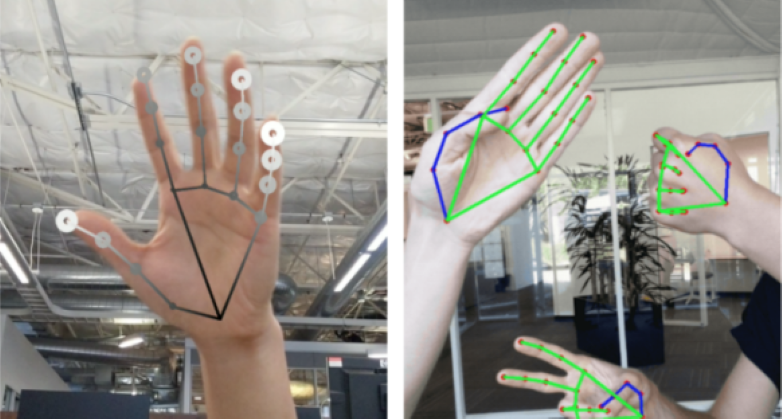
\includegraphics[width=1.0\linewidth]{slike/MediaPipeHandsFigure2.png}
    \caption{Кључне тачке шаке~\cite{DBLP:journals/corr/abs-2006-10214}.}
    \label{fig:kljuchnetachke}
\end{figure}


\textit{MediaPipe hands} решење користи процес машинског учења (енгл. \textit{ML pipeline}) који се састоји од два модела машинског учења:
\begin{itemize}
  \item Први модел је детектор шаке. Модел обрађује целокупну слику са улаза, детектује шаке и враћа оријентисани правоугаоник који обухвата шаку.
  \item Други модел је модел за препознавање карактеристичних тачака шаке. Улаз овог модела је исечак целокупне слике, односно правоугаоник који обухвата само шаку добијен помоћу претходно поменутог детектора шаке. Овај модел враћа 3Д кључне тачке шаке.
\end{itemize}

Прецизно исечена слика длана која представља улазни податак код модела за препознавање карактеристичних тачака шаке умногоме смањује потребу за проширивањем скупа података које подразумева ротације, транслације и скалирање слика (енгл. \textit{data augmentation}) и даје могућност мрежи да већину својих капацитета користи у циљу повећања прецизности одређивања карактеристичних тачака.










\subsection{Детектор шаке}
За детекцију почетних положаја шаке коришћен jе \textit{Single shot detector} SSD модел~\cite{DBLP:journals/corr/LiuAESR15} сличан \textit{BlazeFace}-у~\cite{blazeface}. Детекција шака је изузетно сложен задатак који подразумева прављење модела који може да ради са шакама различитих величина и да детектује заклоњене шаке, односно шаке које су делимично сакривене другим објектима (нпр. предметима, другом руком) и делове шаке који су сакривени другим деловима исте шаке (нпр. прсте преко длана).

Уместо тренирања детектора целе шаке, тренира се детектор длана јер је одређивање правоугаоника који обухватају објекте као што су отворене шаке и шаке скупљене у песницу значајно једноставније од детекције шака са прстима у различитим, савијеним и раширеним положајима.

За издвајање карактеристика користи се кодер-декодер сличан као FPN~\cite{lin2016feature}.


Архитектура детектора шаке приказана је на слици~\ref{fig:архитектурадетекторашаке}.

\begin{figure}[H]
    \centering
    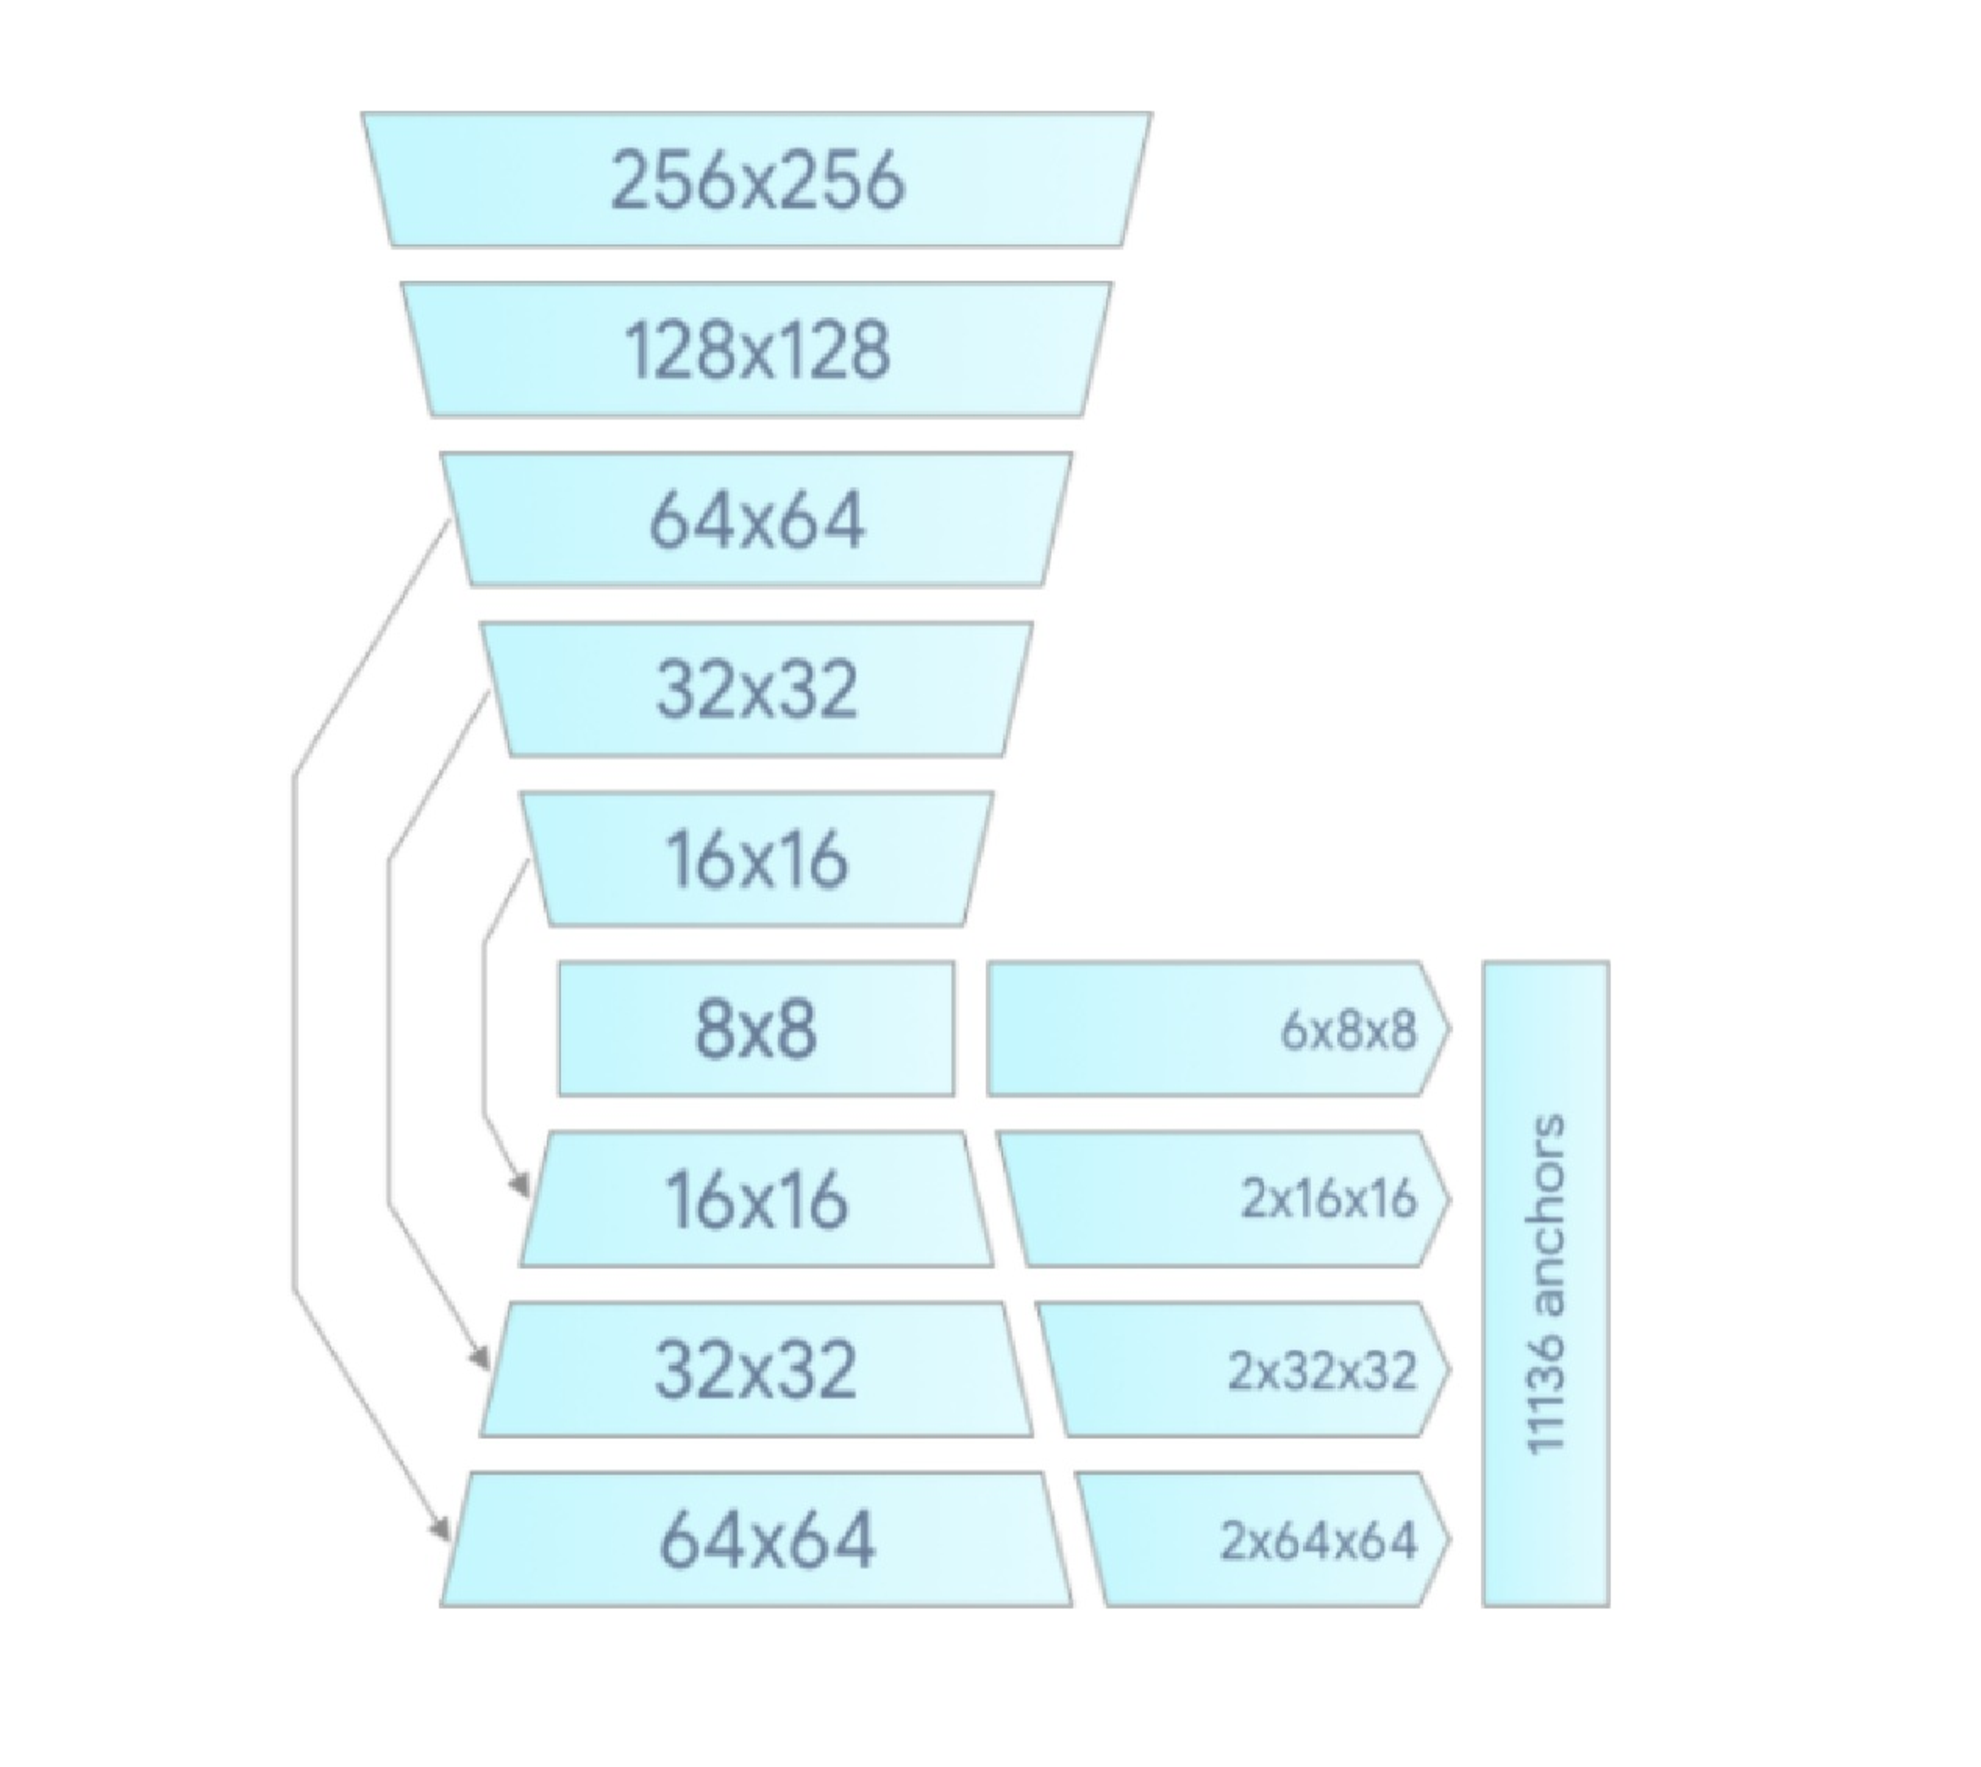
\includegraphics[width=1.0\linewidth]{slike/palm_detector2.pdf}
    \caption{Архитектура модела детектора длана~\cite{DBLP:journals/corr/abs-2006-10214}.}
    \label{fig:архитектурадетекторашаке}
\end{figure}
    

\subsection{Модел за препознавање карактеристичних тачака шаке}

Након што се изврши детекција длана тако што на улаз модела детектора длана долази целокупна слика други модел, модел за препознавање карактеристичних тачака користећи регресију одређује 2.5Д координате за двадесет и једну кључну тачку шаке у оквиру области коју је први модел детектовао као шаку. Модел за препознавање карактеристичних тачака учи како су прсти и зглобови међусобно повезани односно образац који дефинише шаку и на тај начин даје добре резултате и онда када су делови шаке сакривени или се виде само делови прстију. На слици~\ref{fig:slikaландмарк} приказана су три излаза модела за препознавање кључних тачака:

\begin{enumerate}
    \item Двадесет и једна кључна тачка од којих је свака представљена са $x$, $y$ и релативном дубином.
    \item Ознака шаке која дефинише вероватноћу присуства шаке на улазној слици. 
    \item Бинарна класификација која одређује да ли је шака лева или десна.
\end{enumerate}




\begin{figure}[H]
    \centering
    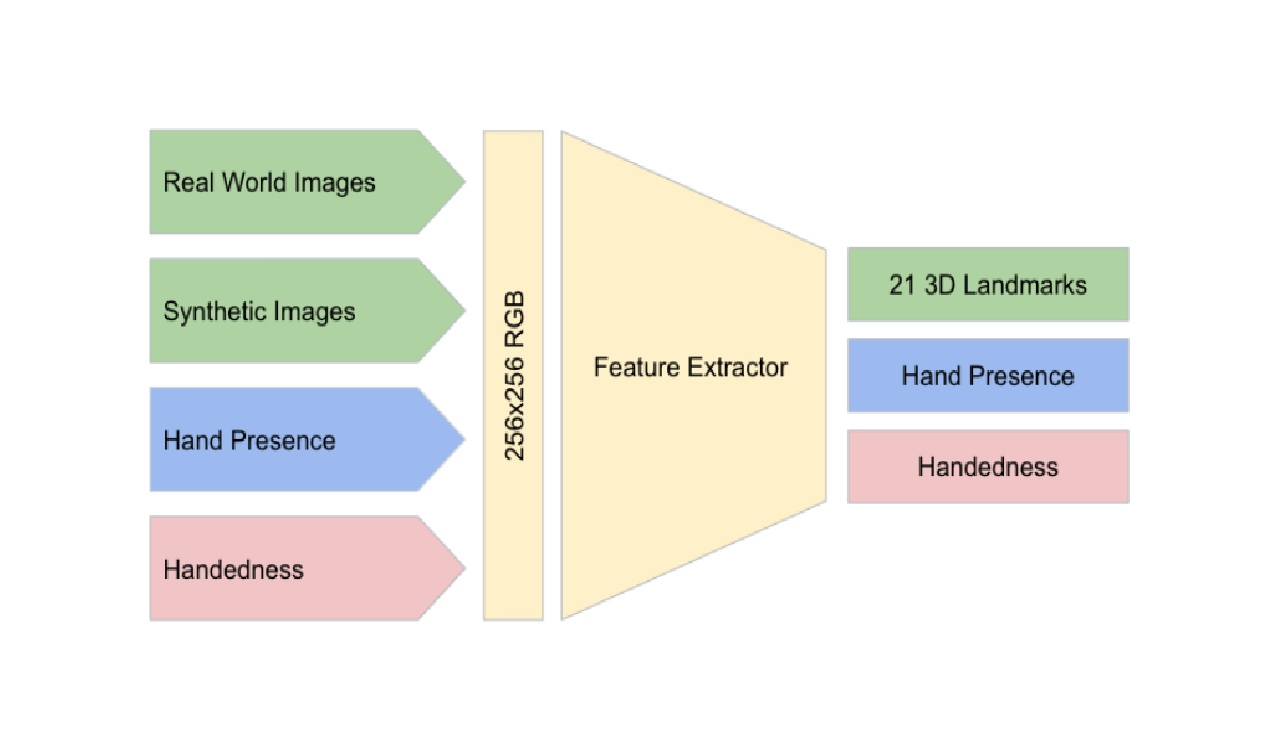
\includegraphics[width=\linewidth]{slike/hand_landmark.jpg}
    \caption{Архитектура модела за препознавање карактеристичних тачака шаке~\cite{DBLP:journals/corr/abs-2006-10214}.}
    \label{fig:slikaландмарк}
\end{figure}



\subsection{Скуп података \textit{MediaPipe hands} решења}

У циљу добијања поузданих података (енгл.  \textit{ground truth data}) направљени су следећи скупови података:

\begin{itemize}
  \item Скуп података који садржи 6 000 разноврсних слика које потичу из различитих делова света, а не из једне земље или једне популације. Осветљења простора у којима су слике прикупљане су различита, а различит је и изглед шака. Ограничење овог скупа података јесте то што не садржи комплексне гестикулације шакама.
  \item Скуп података који садржи 10 000 слика које обухватају различите углове свих физички могућих гестикулација шакама. Недостатак овог скупа података је то што је направљен од слика снимљених од само тридесет људи.
  \item Синтетички скуп података који је направљен генерисањем модела шаке преко различитих позадина коришћењем рачунарског програма (енгл. \textit{rendering}) и пресликавањем тог модела на одговарајуће 3Д координате. Циљ овог метода је још боље обухватање потенцијалних положаја шаке.
\end{itemize}

Примерци из скупова података коришћених за тренирање модела приказани су на слици~\ref{fig:slika}.

\begin{figure}[H]
    \centering
    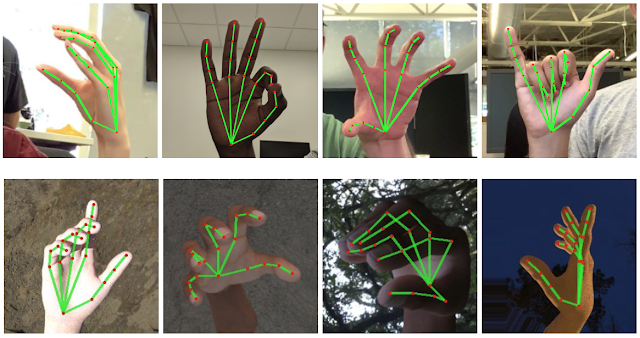
\includegraphics[width=1.0\linewidth]{slike/hand_crops2.png}
    \caption{Примерци из скупова података коришћених за тренирање модела~\cite{DBLP:journals/corr/abs-2006-10214}.}
    \label{fig:slika}
\end{figure}

\subsection{\textit{MediaPipe} граф}

Коришћењем \textit{MediaPipe} софтверског оквира, систем који омогућава праћење шака може да се реализује у виду графа који се састоји од модуларних компонената. 
\textit{MediaPipe} граф за праћење шаке приказан је на слици~\ref{fig:slikagraf}. Граф се састоји од два подграфа, од којих је један подграф за детекцију шаке - HandDetection, а други за израчунавање координата кључних тачака шаке - HandLandmark.

Кључно побољшање које \textit{MediaPipe }обезбеђује јесте то што се детектор шаке користи само по потреби (прилично ретко) и на тај начин се значајно смањују израчунавања. Ово се постиже извођењем позиција шаке тренутних статичних слика видеа (енгл. \textit{frames}) на основу већ израчунатих кључних тачака шаке из претходне статичне слике. На тај начин се уклања потреба за применом детектора шаке на свакој статичној слици.

У циљу веће поузадности, модел за праћење шаке на излазу даје додатну скаларну вредност која показује степен поверења да је шака заиста присутна. Модел за детекцију шаке се примењује поново на следећој статичној слици само када степен поверења падне испод одређеног прага. 


\begin{figure}[H]
    \centering
    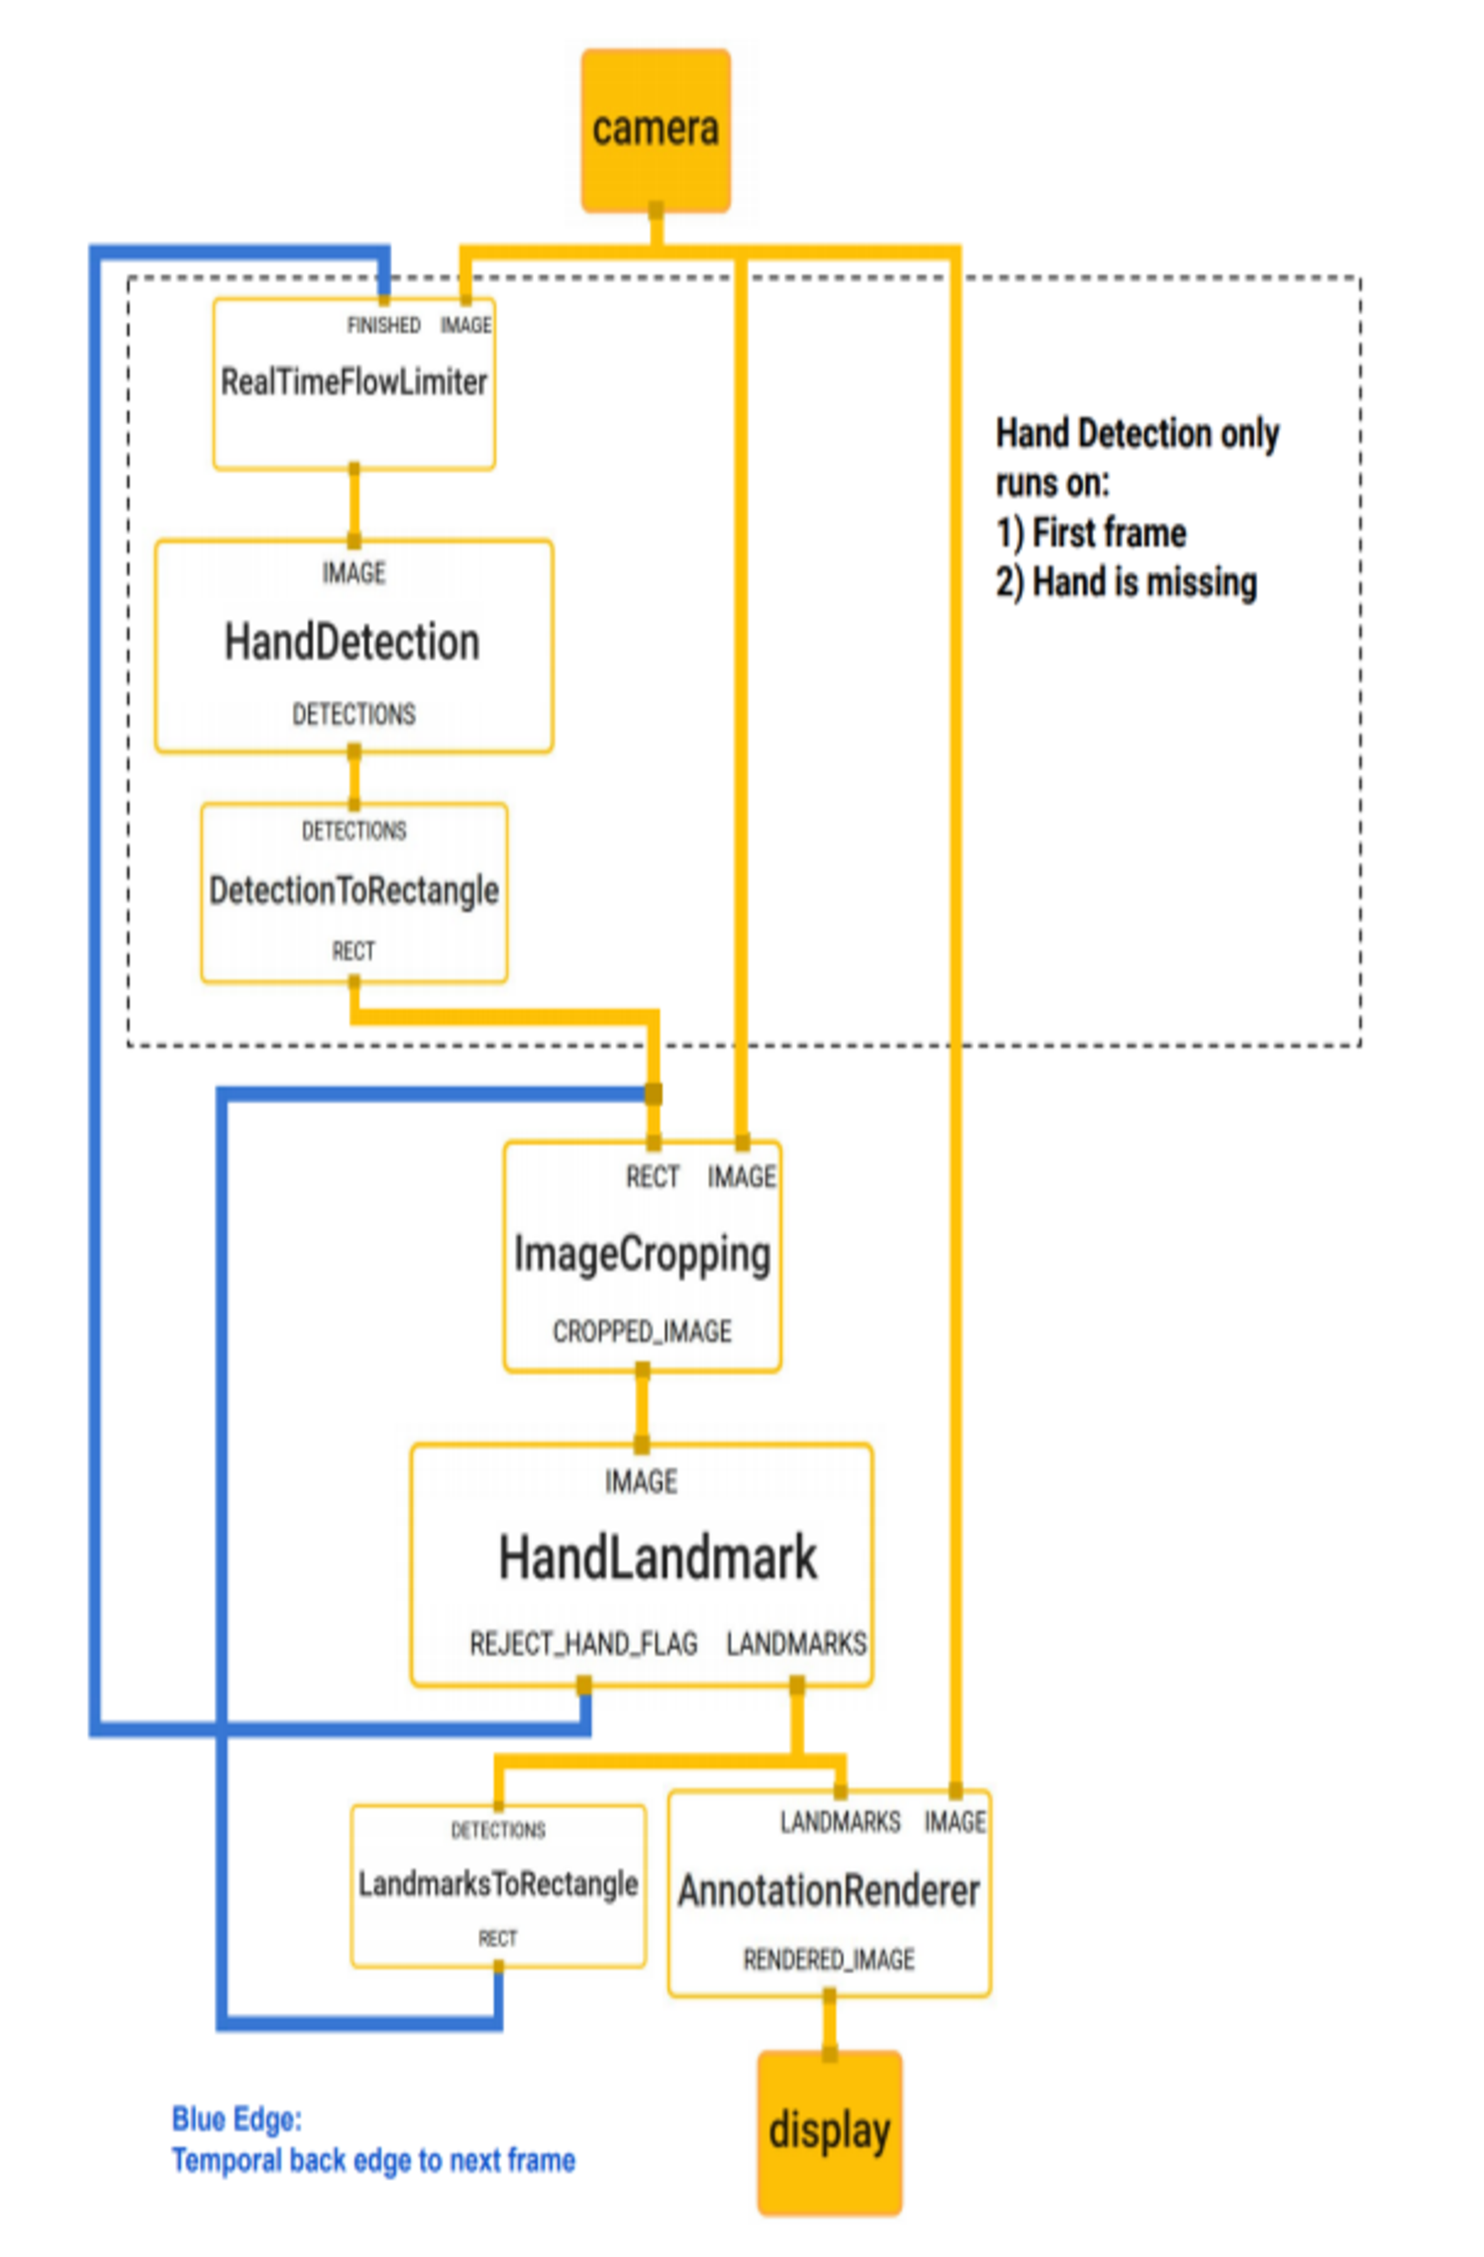
\includegraphics[width=\linewidth, height=0.93\textheight]{slike/mediapipe.pdf}
    \caption{\textit{MediaPipe} граф за праћење шаке~\cite{DBLP:journals/corr/abs-2006-10214}.}
    \label{fig:slikagraf}
\end{figure}
\section{Имплементација система за препознавање гестикулација шаком}

За имплементацију система за препознавање шаке и гестикулација шаком на видео снимцима са веб камере коришћен je програмски језик Пајтон и \textit{MediaPipe} и \textit{Keras} библиотеке. Систем је способан да
препозна осам гестикулација приказаних на слици~\ref{fig:osamgestikulacija}, укључујући отворену шаку, шаку са пруженим палцем на горе (енгл. \textit{like}), знак победе, рокенрол знак, круг, песницу, показивач и шаку са пруженим палцем на доле (енгл. \textit{dislike}). На слици~\ref{fig:slikadelovi} приказани су делови овог система. Систем за препознавање чини део у коме се прво препознају кључне тачке на шаци, односно \textit{MediaPipe} фрејмворк. Други део система чини потпуно повезана неуронска мрежа (енгл. \textit{fully-connected feedforward neural network}) која као улазне податке користи координате кључних тачака шаке из претходног дела и на основу њих класификује гестикулације. Имплементација система је делимично инспирисана алгоритмом описаним у \textit{README} датотеци репозиторијума отвореног кода \textit{kinivi/hand-gesture-recognition-mediapipe}.

RGB слика приказана на слици~\ref{fig:slikadelovi} представља улаз у целокупан систем~\cite{app11083418}. RGB (од енглеског \textbf{R}ed, \textbf{G}reen, \textbf{B}lue, у преводу „црвена, зелена, плава”) је модел боја код којег се сабирањем три основне боје на различите начине добијају све остале боје. RGB слике се састоје од више пиксела, а сваки пиксел садржи три канала: црвени, плави и зелени. Интензитет црвене, зелене и плаве боје у пикселу одређује резултујућу боју пиксела.

\begin{figure}[H]
    \centering
    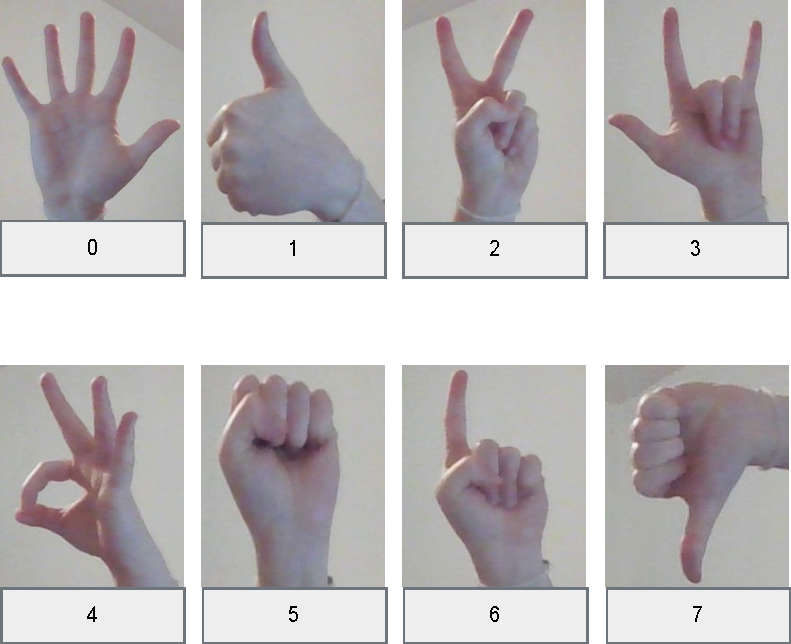
\includegraphics[width=0.9\linewidth]{slike/labels.drawio.pdf}
    \caption{Осам гестикулација.}
    \label{fig:osamgestikulacija}
\end{figure}
 

\vspace{3em}

\begin{figure}[H]
    \centering
    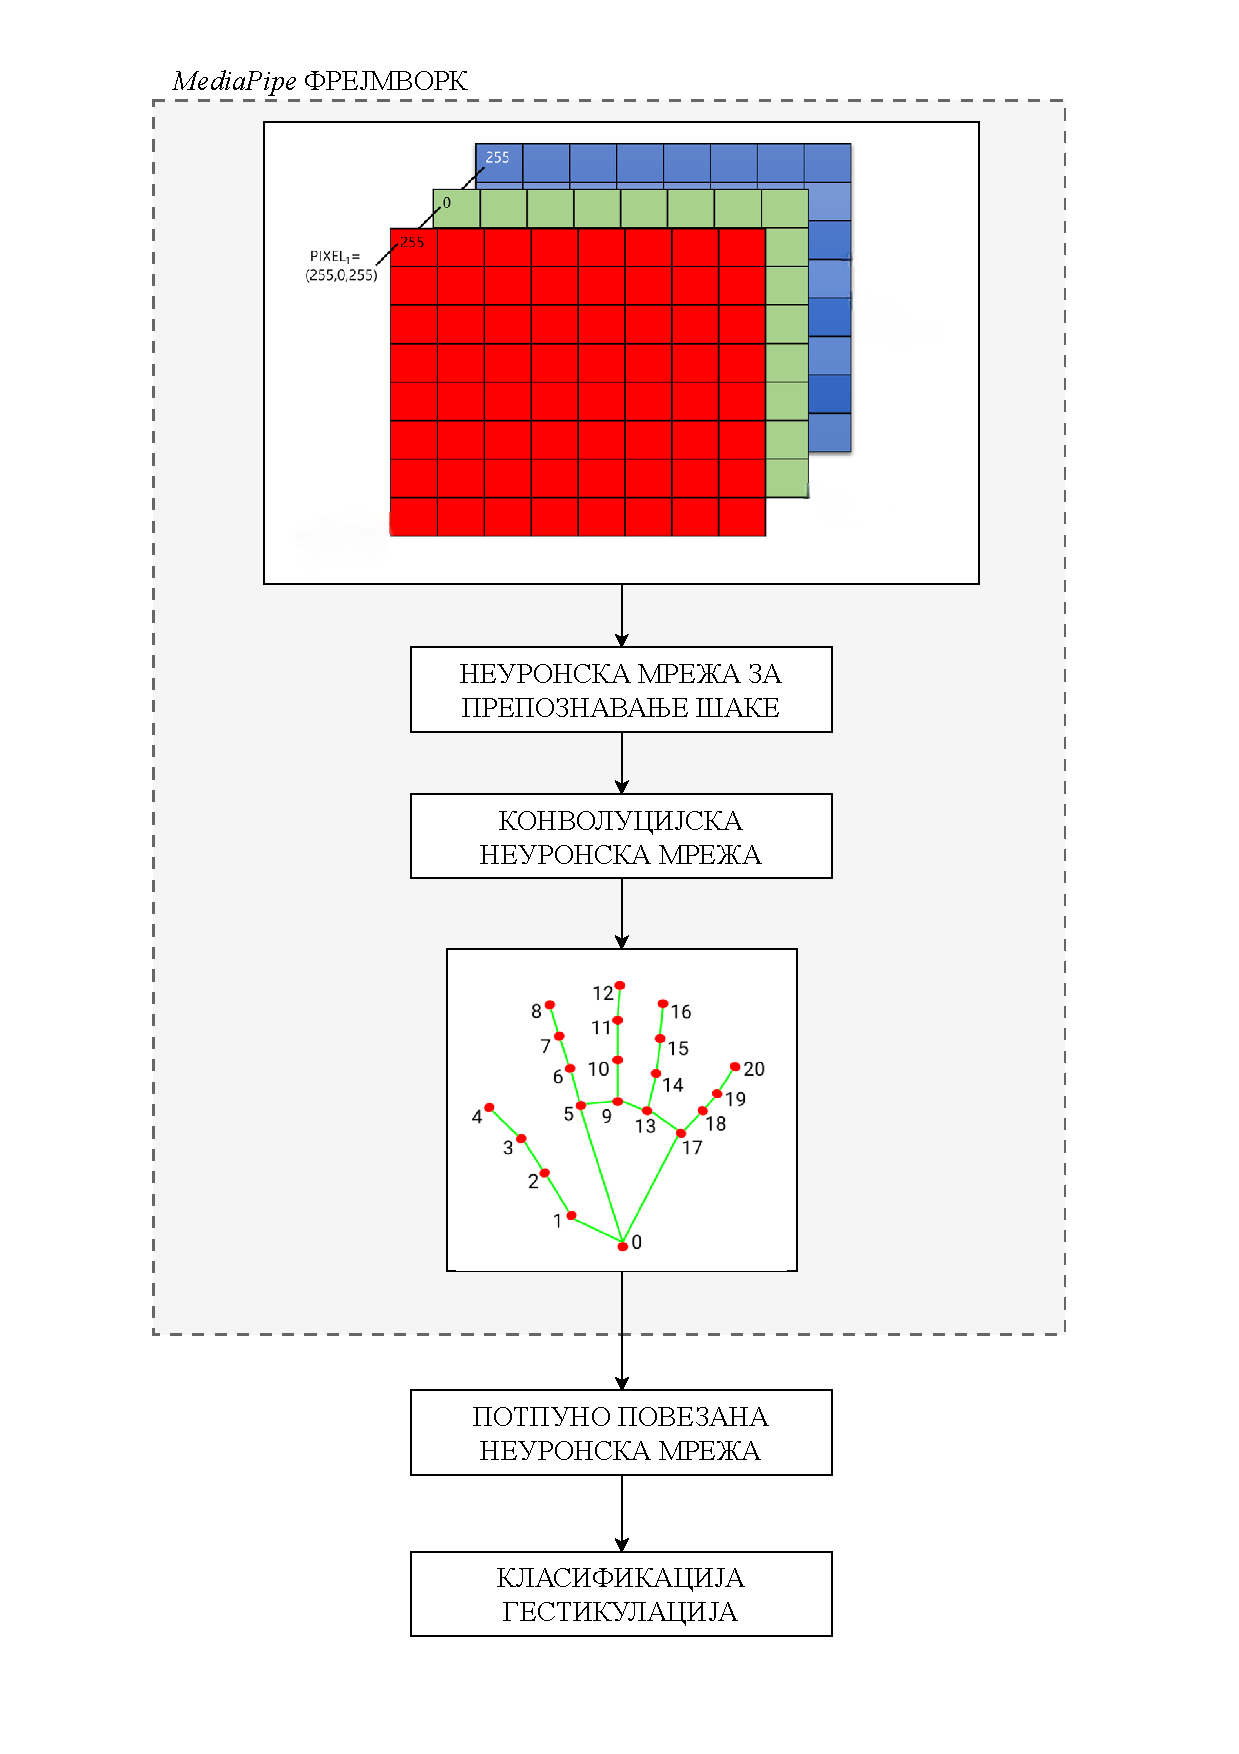
\includegraphics[width=\linewidth]{slike/ДЕЛОВИ_СИСТЕМА8.drawio.pdf}
    \caption{Делови система за препознавање гестикулација шаком.}
    \label{fig:slikadelovi}
\end{figure}

\vspace{2em}
Листинг~\ref{lst:py:main.py} представља главну датотеку пројекта која може да се покрене на два начина, односно има два режима рада. У првом режиму рада датотека омогућава стварање скупа података за неуронску мрежу система за препознавање гестикулација шаком, а у другом режиму рада датотека покреће систем.

Покретањем датотеке у првом режиму рада укључује се камера и отвара се прозор камере на екрану рачунара. Коришћење \textit{MediaPipe} библиотеке омогућава детекцију шаке и кључних тачака шаке. На слици~\ref{fig:slikaшемашаке} приказана је шема свих кључних тачака шаке, a на слици~\ref{fig:slikaпрозоршака} прозор који се отвара покретањем поменуте датотеке у првом режиму рада. За прикупљање података у облику координата које дефинишу одређену гестикулацију потребно је испред камере приказати гестикулацију и притиснути одговарајући тастер на тастатури. Гестикулације су повезане са тастерима на следећи начин:

\begin{itemize}
  \item Отворена шака - тастер 0
  \item Шака са пруженим палцем на горе - тастер 1
  \item Знак победе - тастер 2
  \item Рокенрол знак - тастер 3
  \item Круг - тастер 4
  \item Песница - тастер 5
  \item Показивач - тастер 6
  \item Шака са пруженим палцем на доле - тастер 7
\end{itemize}


\vspace{2em}

\begin{lstlisting}[language=Python, caption={Имплементација система за препознавање гестикулација.}, label={lst:py:main.py}]
import os
import mediapipe as mp
import cv2
import time # added per Copilot suggestion 

from points import save_data, directory
from coordinates import Coordinates
from keras import models
from numpy import loadtxt

MODEL = r'model_8_both_hands_19_1_v3.h5'
REALTIME_DATA = r'data\temp\realtimedata.csv' 

def run_mediapipe(mode):
    mp_drawing = mp.solutions.drawing_utils
    mp_drawing_styles = mp.solutions.drawing_styles
    mp_hands = mp.solutions.hands
    
    row_num = 0
    
    cap = cv2.VideoCapture(0)
    with mp_hands.Hands(
        model_complexity=0,
        min_detection_confidence=0.5,
        min_tracking_confidence=0.5) as hands:
      
      prediction = 5
      gesture = ""  # added per Copilot suggestion
      gesture_time = 0  # Track when gesture was detected # added per Copilot suggestion 
       
      while cap.isOpened():
        success, image = cap.read()
        if not success:
          print("Ignoring empty camera frame.")
          # If loading a video, use 'break' instead of 'continue'.
          continue
    
        image.flags.writeable = False
        image = cv2.cvtColor(image, cv2.COLOR_BGR2RGB)
        results = hands.process(image)
        
        # Draw the hand annotations on the image.
        image.flags.writeable = True
        image = cv2.cvtColor(image, cv2.COLOR_RGB2BGR)
        
        k = cv2.waitKey(5) & 0xFF
        
        if results.multi_hand_landmarks:
          for hand_landmarks in results.multi_hand_landmarks:
            mp_drawing.draw_landmarks(
                image,
                hand_landmarks,
                mp_hands.HAND_CONNECTIONS,
                mp_drawing_styles.get_default_hand_landmarks_style(),
                mp_drawing_styles.get_default_hand_connections_style())
            
            if mode == 0:
          
              if k == 48 or k == 49 or k == 50 or k == 51 or k == 52 or k == 53 or k == 54 or k == 55:
                  
                match k:
                  case 48:
                    pressed_key = 0
                  case 49:
                    pressed_key = 1
                  case 50:
                    pressed_key = 2
                  case 51:
                    pressed_key = 3
                  case 52:
                    pressed_key = 4
                  case 53:
                    pressed_key = 5
                  case 54:
                    pressed_key = 6
                  case 55:
                    pressed_key = 7
                    
                save_data(hand_landmarks, mode)
                coord = Coordinates(mode, pressed_key)
                coord.twod_coordinates()
                row_num = row_num + 1
                print("{} row(s) added".format(row_num))
                
                directory(mode)
            
            elif mode == 1: 
              
              # press 's' to save coordinate; ascii code 
              if k == 115:
                print("App in the form for end users")
                
                save_data(hand_landmarks, mode)
                
                coord = Coordinates(mode)
                coord.twod_coordinates()
                
                model = models.load_model(MODEL)
                
                realtime_data = loadtxt(REALTIME_DATA, delimiter=',')
                realtime_data = realtime_data.reshape(1, 42)
                              
                prediction = model.predict(realtime_data)
                
                label = prediction.argmax()
                
                match label:
                    case 0:
                      gesture = "open palm" 
                    case 1:
                      gesture = "like"
                    case 2:
                      gesture = "victory"
                    case 3:
                      gesture = "rock and roll"
                    case 4:
                      gesture = "ok"
                    case 5:
                      gesture = "closed fist"
                    case 6:
                      gesture = "pointer"
                    case 7:
                      gesture = "dislike"
                
                gesture_time = time.time()  # Record when gesture was detected # added per Copilot suggestion
                directory(mode)
                
                f = open(REALTIME_DATA, "w+")
                f.close()

                os.remove(REALTIME_DATA)

        if mode == 0:
          # Flip the image horizontally for a selfie-view display.
          cv2.imshow('Gesture recognition', cv2.flip(image, 1))
          
        elif mode == 1:
          if gesture and (time.time() - gesture_time < 1): # added per Copilot suggestion
            
            # Generated/refactored with Copilot
            # Get text size for background rectangle
            text = f'{gesture}'
            font = cv2.FONT_HERSHEY_SIMPLEX
            font_scale = 1.5
            thickness = 2
            (text_width, text_height), baseline = cv2.getTextSize(text, font, font_scale, thickness)
            
            # Draw background rectangle with padding
            padding = 10
            x, y = 25, 42
            cv2.rectangle(image, 
                         (x - padding, y - text_height - padding), 
                         (x + text_width + padding, y + baseline + padding), 
                         (255, 255, 255),  # White background
                         -1)  # Filled rectangle
            
            # Draw text on top of rectangle
            image = cv2.putText(image, text, (x, y), font, font_scale, (103, 51, 25), thickness, cv2.LINE_AA)
            # Generated/refactored with Copilot
          cv2.imshow('Gesture recognition', image)
          
        if k == 27:
          break   
      
    cap.release()
    
if __name__ == "__main__":
  
    """File that will present created dataset is referenced in coordinates.py
          with open(DATASET, "a") as f: ...
          
    In order to collect data press '0-7' on the keybaord depending on the label/class
    you are collecting. 
    """
    
    # following print statements were refactored using Copilot
    
    print("\n" + "="*60)
    print("GESTURE RECOGNITION SYSTEM")
    print("="*60)
    print("Select mode:")
    print("  * Mode 0 - Creates custom dataset for ML model")
    print("  * Mode 1 - Starts application for end users")
    print("="*60 + "\n")
    
    mode = input("Enter mode (0 or 1): ")
    
    if mode == '0':
      run_mediapipe(0)
    elif mode == '1':
      run_mediapipe(1)
\end{lstlisting}

Линије кода из листинга~\ref{lst:py:main.py} додате коришћењем \textit{GitHub Copilot} асистента за програмирање заснованог на вештачкој интелигенцији обележене су коментаром: \begin{verbatim}# added per Copilot suggestion \end{verbatim} Питања постављана асистенту:
\begin{enumerate}
    \item У једној од верзија кода систем је на прозору камере исписивао назив гестикулације који је остајао исписан све док систем не препозна следећу гестикулацију. Питање постављено асистенту је гласило: „Да ли можеш да унапредиш код тако да се након једне секунде назив гестикулације коју је систем препознао избрише?”
    \item „Да ли можеш да нацрташ правоугаоник око назива препознате гестикулације?” 
    \item „Да ли можеш да средиш текст који се исписује у терминалу при покретању датотеке тако да визуелно изгледа сложеније и лепше?”
\end{enumerate}

Променљива \verb |hand_landmarks| чува $x$, $y$ и $z$ вредности сваке тачке у формату приказаном у листингу~\ref{lst:py:hand_landmarks}.

\vspace{2em}
\begin{figure}[H]
\captionof{lstlisting}{Променљива \texttt{hand\_landmarks}.}
\label{lst:py:hand_landmarks}

\noindent
\begin{minipage}[t]{0.32\textwidth}
\begin{lstlisting}[numbers=none, xleftmargin=0.5cm, frame=none, basicstyle=\ttfamily\normalsize\linespread{1.25}\selectfont]
landmark {                      
  x: 0.209368929
  y: 0.850705326
  z: 9.19832299e-009
}
landmark {
  x: 0.269909322
  y: 0.80474925
  z: -0.0172585528
}
landmark {
  x: 0.314091116
  y: 0.739561558
  z: -0.0321756601
}
landmark {
  x: 0.340909064
  y: 0.679775298
  z: -0.0486022085
}
landmark {
  x: 0.367133737
  y: 0.640210152
  z: -0.0658991411
}
landmark {
  x: 0.259260893
  y: 0.629035056
  z: -0.0220199116
}
landmark {
  x: 0.278147548
  y: 0.539927423
  z: -0.0390892252
}
\end{lstlisting}
\end{minipage}
\hfill
\begin{minipage}[t]{0.32\textwidth}
\begin{lstlisting}[numbers=none, xleftmargin=0.5cm, frame=none, basicstyle=\ttfamily\normalsize\linespread{1.25}\selectfont]
landmark {
  x: 0.286446601
  y: 0.48600018
  z: -0.0510048345
}
landmark {
  x: 0.291387171
  y: 0.43847245
  z: -0.0607785
}
landmark {
  x: 0.21715343
  y: 0.621121764
  z: -0.0310199913
}
landmark {
  x: 0.225248843
  y: 0.523398519
  z: -0.0461683
}
landmark {
  x: 0.229123116
  y: 0.465477943
  z: -0.059615992
}
landmark {
  x: 0.229885921
  y: 0.413204253
  z: -0.0715518445
}
landmark {
  x: 0.179624125
  y: 0.635847449
  z: -0.0424561352
}
\end{lstlisting}
\end{minipage}
\hfill
\begin{minipage}[t]{0.32\textwidth}
\begin{lstlisting}[numbers=none, xleftmargin=0.5cm, frame=none, basicstyle=\ttfamily\normalsize\linespread{1.25}\selectfont]
landmark {
  x: 0.170684814
  y: 0.551132858
  z: -0.0596783645
}
landmark {
  x: 0.166142672
  y: 0.497690856
  z: -0.0744622424
}
landmark {
  x: 0.161875442
  y: 0.449028909
  z: -0.0853128135
}
landmark {
  x: 0.144418746
  y: 0.668792307
  z: -0.0562961325
}
landmark {
  x: 0.117199667
  y: 0.608865321
  z: -0.0710861683
}
landmark {
  x: 0.0997032076
  y: 0.571289539
  z: -0.0812236592
}
landmark {
  x: 0.0847765654
  y: 0.533703685
  z: -0.0890323892
}
\end{lstlisting}
\end{minipage}
\end{figure}



\begin{figure}[H]
    \centering
    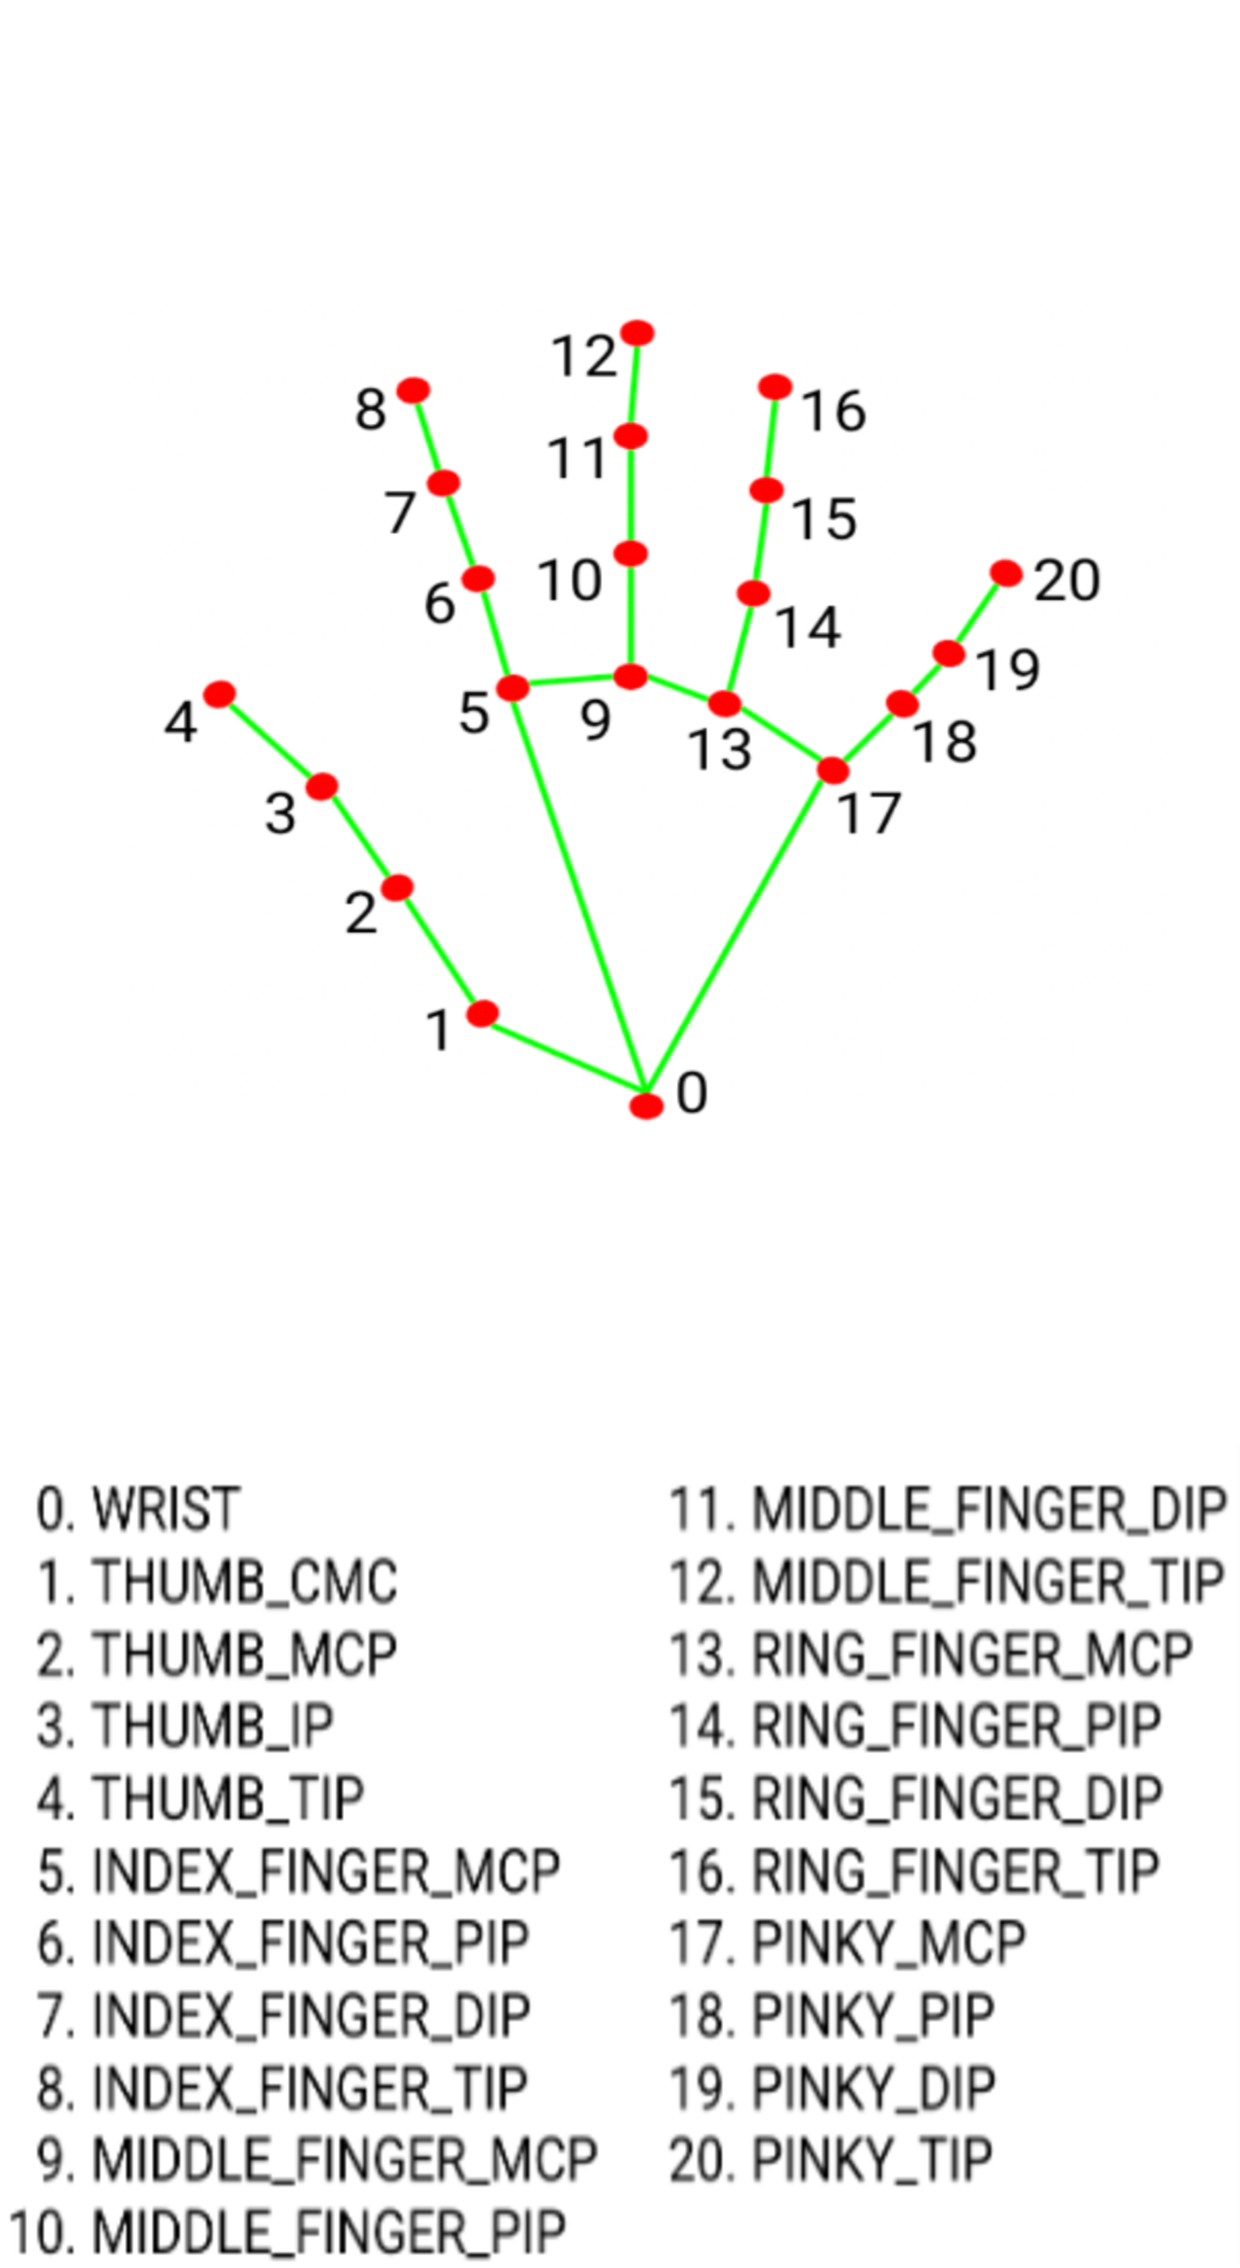
\includegraphics[width=0.8\linewidth]{slike/pointsnew9.pdf}
    \caption{Шематски приказ кључних тачака шаке~\cite{mediapipehands}.}
    \label{fig:slikaшемашаке}
\end{figure}


\begin{figure}[H]
    \centering
    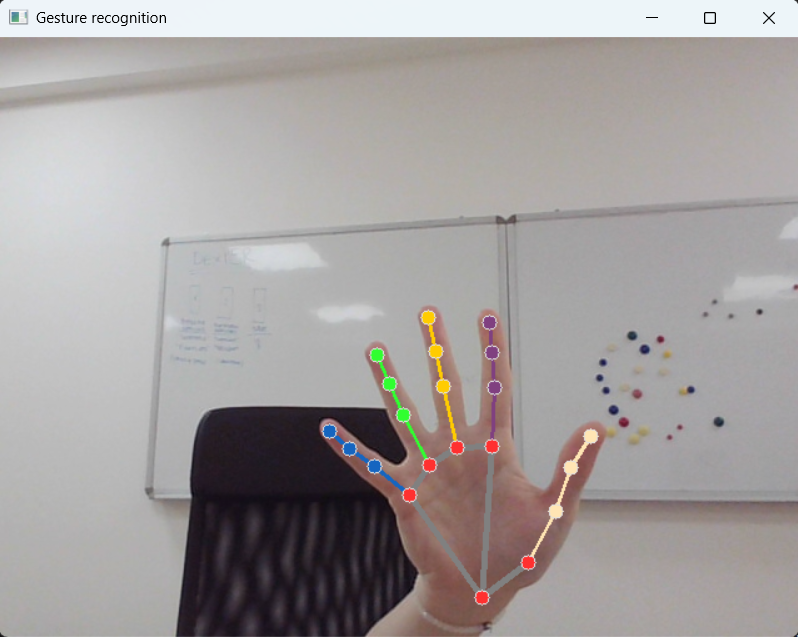
\includegraphics[width=\linewidth]{slike/хејхеј.png}
    \caption{Детекција кључних тачака шаке у реалном времену.}
    \label{fig:slikaпрозоршака}
\end{figure}



\subsection{Обрада улазних података}

Обрада улазних података прво подразумева пројекцију координата сваке кључне тачке шаке из тродимензионалног (формат приказан у листингу~\ref{lst:py:hand_landmarks}) у дводимензионални простор, а затим нормализацију. Како би се извршила пројекција координата из тродимензионалног у дводимензионални простор потрбено је урадити калибрацију камере коришћене у систему за препознавање гестикулација.

\subsubsection{Калибрација камере}

Пре пројекције координата из тродимензионалног у дводимензионални простор потребно је урадити калибрацију камере, пронаћи матрицу камере и параметре дисторзије. Матрица камере је јединствена за сваку камеру и дефинише се као матрица димензија 3x3: 

\begin{equation} 
\begin{bmatrix}
f_x & 0 & c_x\\
0 & f_y & c_y\\
0 & 0 & 1
\end{bmatrix}
\end{equation}

Пројекција 3Д тачке $P_w$ на раван слике коришћењем модела \textit{pinhole} камере (једноставне камере без сочива са малим отвором бленде~\cite{UjfalusiTrpovski2025}) приказана је на слици~\ref{fig:pinholecamera}.

\begin{figure}[H]
    \centering
    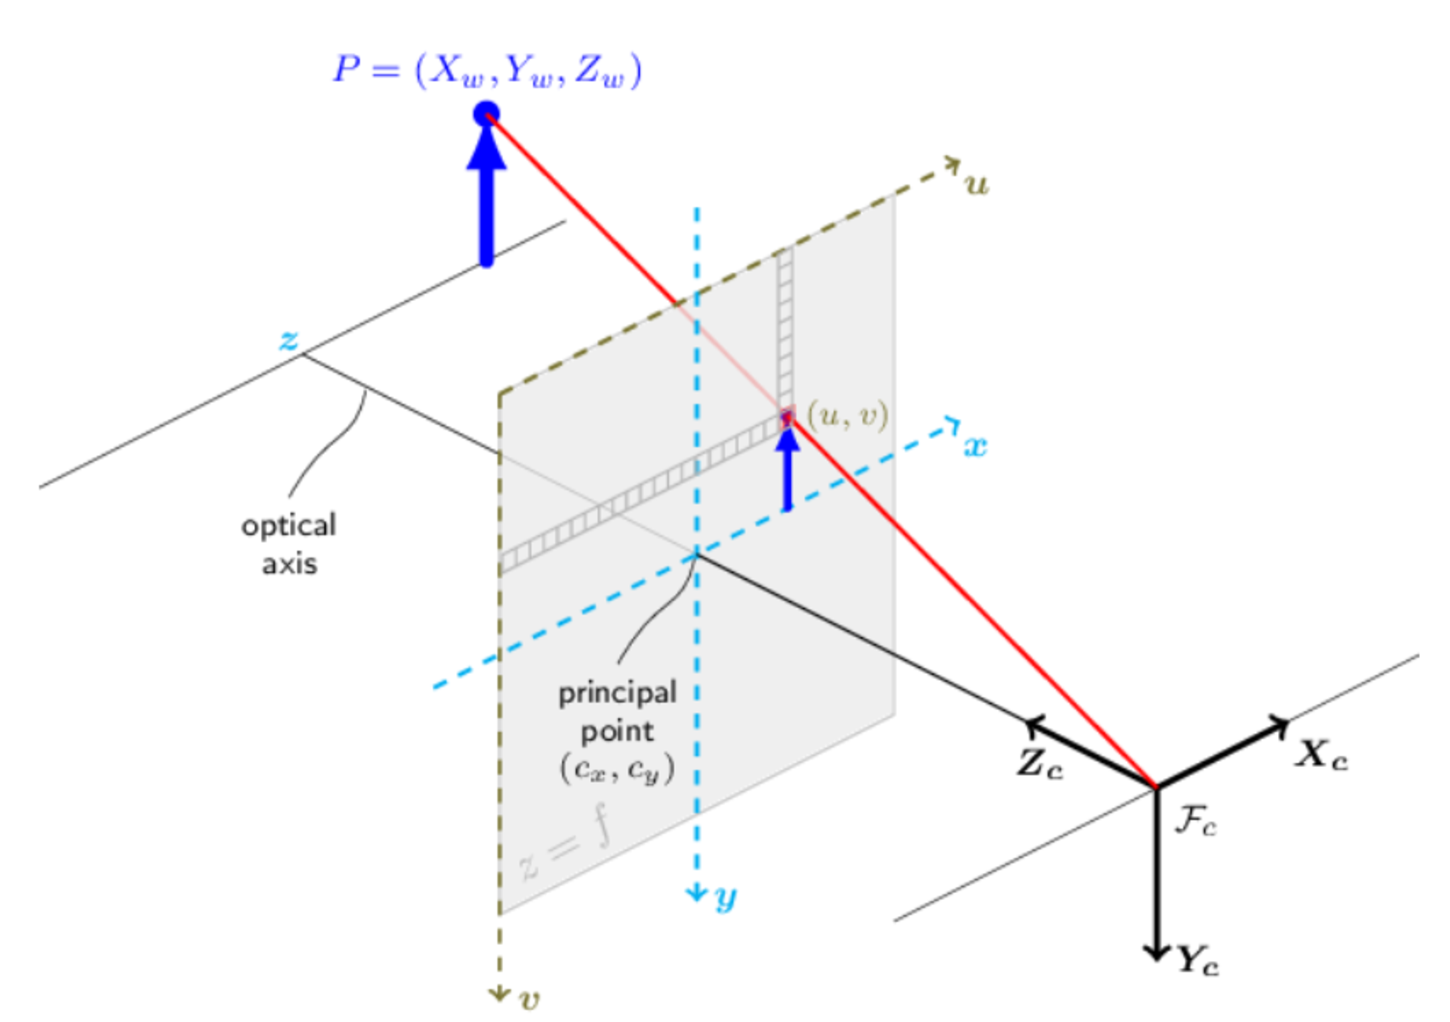
\includegraphics[width=\linewidth]{slike/camera_model3.pdf}
    \caption{Модел \textit{pinhole} камере~\cite{OpenCVCalib3d}.}
    \label{fig:pinholecamera}
\end{figure}



\begin{lstlisting}[language=Python, caption={Имплементација класе за калибрацију камере.}, label={lst:py:cameracalibration}]
import numpy as np
import cv2 as cv
import glob
import os

class CameraCalibration:
    
    def __init__(self,
                 chessboard_size = (7,7),   # number of corners on the chessboard in the width and height
                 frame_size = (1280,720)):
        
        self.chessboard_size = chessboard_size
        self.frame_size = frame_size
        self.criteria = (cv.TERM_CRITERIA_EPS + cv.TERM_CRITERIA_MAX_ITER, 30, 0.001)
        self.objp = np.zeros((chessboard_size[0] * chessboard_size[1], 3), np.float32)
        self.objp[:,:2] = np.mgrid[0:chessboard_size[0], 0:chessboard_size[1]].T.reshape(-1,2)
        self.objpoints = []
        self.imgpoints = []
        
    def load_images(self, path):
        images = glob.glob(path)
        return images
        
    def detect_corners(self, images):
        for fname in images:
            print(fname)
            img = cv.imread(fname)
            gray = cv.cvtColor(img, cv.COLOR_BGR2GRAY)
            
            # Find the chess board corners
            ret, corners = cv.findChessboardCorners(gray, self.chessboard_size, None)
            
            # If found, add object points, image points (after refining them)
            if ret == True:
                self.objpoints.append(self.objp)
                corners2 = cv.cornerSubPix(gray,corners, (11,11), (-1,-1), self.criteria)
                self.imgpoints.append(corners2) # corners2 or corners?
                
                # Draw and display the corners
                cv.drawChessboardCorners(img, self.chessboard_size, corners2, ret)
                cv.imshow('img', img)
                cv.waitKey(1000)
    
        cv.destroyAllWindows()
        
        return self.objpoints, self.imgpoints
    
    def calibrate_camera(self, objpoints, imgpoints):
        ret, mtx, dist, rvecs, tvecs = cv.calibrateCamera(objpoints, imgpoints, self.frame_size, None, None)

        print("Camera Calibrated: ", ret)
        print("\nCamera Matrix:\n", mtx)
        print("\nDistortion Parameters:\n", dist)
        print("\nRotation Vectors:\n", rvecs)
        print("\nTranslation Vectors:\n", tvecs)
        
        return mtx, dist, rvecs, tvecs
        
        
    def undistort_image(self, image_path, mtx, dist, images_folder, objpoints, imgpoints, rvecs, tvecs):
        img = cv.imread(image_path)
        h,  w = img.shape[:2]
        newcameramtx, roi = cv.getOptimalNewCameraMatrix(mtx, dist, (w,h), 1, (w,h))

        # undistort - I
        dst = cv.undistort(img, mtx, dist, None, newcameramtx)
        # crop the image
        x, y, w, h = roi
        dst = dst[y:y+h, x:x+w]
        # cv.imwrite('calibresult1.jpg', dst)
        cv.imwrite(os.path.join(images_folder, 'calibresult1.jpg'), dst)

        # undistort - II
        mapx, mapy = cv.initUndistortRectifyMap(mtx, dist, None, newcameramtx, (w,h), 5)
        dst = cv.remap(img, mapx, mapy, cv.INTER_LINEAR)
        # crop the image
        x, y, w, h = roi
        dst = dst[y:y+h, x:x+w]
        # cv.imwrite('calibresult2.jpg', dst)
        cv.imwrite(os.path.join(images_folder, 'calibresult2.jpg'), dst)

        # Re-projection Error

        mean_error = 0
        for i in range(len(objpoints)):
            imgpoints2, _ = cv.projectPoints(objpoints[i], rvecs[i], tvecs[i], mtx, dist)
            error = cv.norm(imgpoints[i], imgpoints2, cv.NORM_L2)/len(imgpoints2)
            mean_error += error
        
        print( "total error: {}".format(mean_error/len(objpoints)) )
    
\end{lstlisting}

\vspace{2em}
За проналажење унутрашњих и спољашних параметара матрице потребно је користити слике објеката са добро дефинисаним обрасцима односно слике објеката са геомтријом чије карактеристичне тачке могу тачно да се детектују на слици. На пример, објекти које чине равне линије, прави углови и иста растојања. У овом пројекту коришћене су слике шаховске табле.

Резултат методе \verb |detect_corners()| из листинга~\ref{lst:py:cameracalibration} приказан је на слици~\ref{fig:slikaшах}.

\begin{figure}[H]
    \centering
    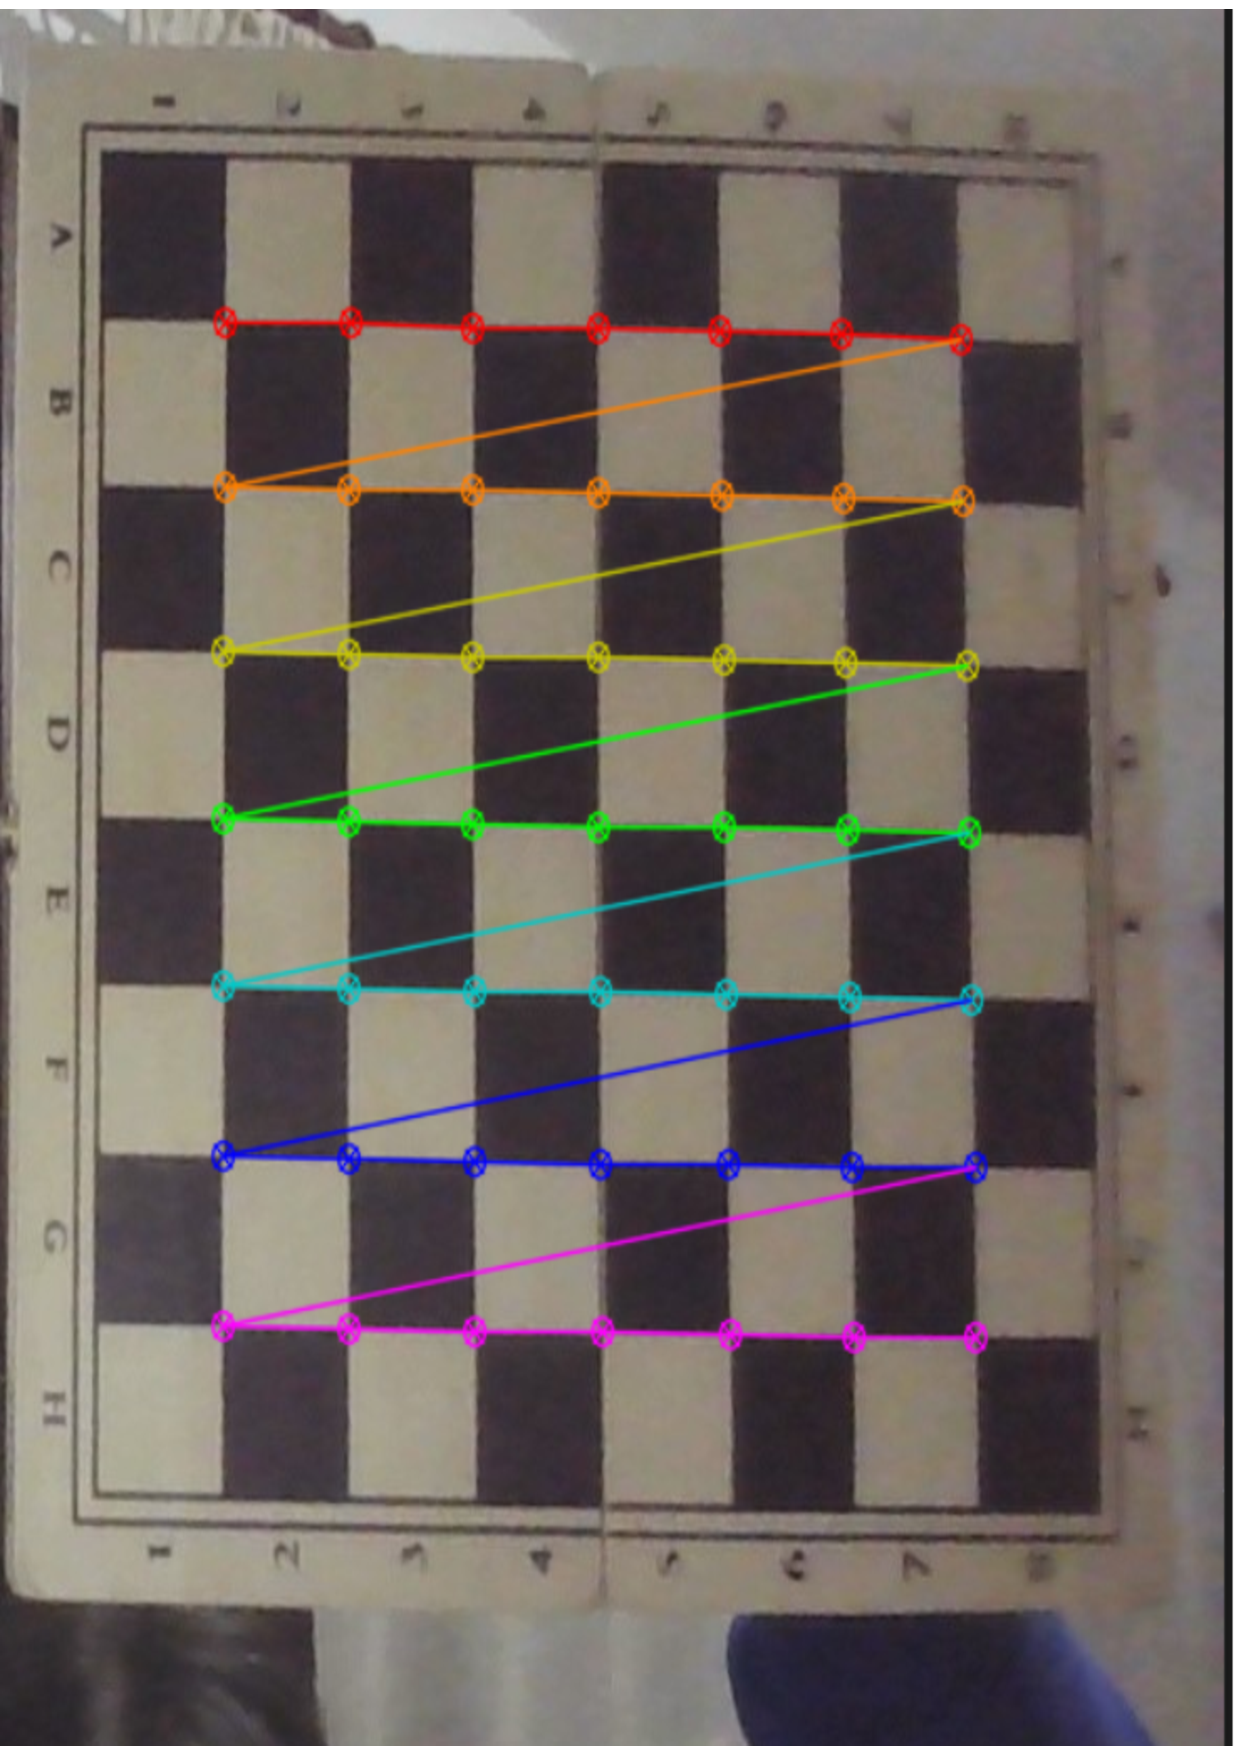
\includegraphics[width=0.8\linewidth]{slike/calibration4.pdf}
    \caption{Шаховска табла коришћена за калибрацију камере.}
    \label{fig:slikaшах}
\end{figure}

Метода \verb |save_data()| приказана у листингу~\ref{lst:py:points.py} позива се у линији 79 у главној 
датотеци приказаној у листингу~\ref{lst:py:main.py} и њој се прослеђује променљива \verb|hand_landmarks| приказана у листингу~\ref{lst:py:hand_landmarks}.

Она привремено чува 3Д координате сваке тачке у \texttt{.npy} датотеци на путањи {\small\texttt{FILEPATH}}. 


\begin{lstlisting}[caption={Структура \texttt{.npy} датотеке.}, label={lst:py:npy}, numbers=none, xleftmargin=3cm, frame=none]
[2.62975365e-01 7.30098128e-01 8.36784864e-09]
\end{lstlisting}

За сваку тачку биће напрвљена \texttt{.npy} датотека, а након једног проласка кроз \texttt{for} петљу биће напрвљена двадесет и једна датотека \texttt{(array1.npy \ldots\ array21.npy)} на путањи \texttt{FILEPATH}.

\begin{lstlisting}[language=Python, caption={Имплементација методе за привремено чување 3Д координата кључних тачака шаке и методе за брисање тих координата након завршетка обраде података.}, label={lst:py:points.py}]
import posixpath
import re
import os

from numpy import save

FILEPATH = r'data\temp\mode0'
FILEPATH_MODE1 = r'data\temp\mode1'

def save_data(hand_landmarks, mode):

    for i in range(21):
      coordinates = {}
        
      point = hand_landmarks.landmark[i]
      
      coordinates.setdefault(i, []).append(point.x)
      coordinates.setdefault(i, []).append(point.y)
      coordinates.setdefault(i, []).append(point.z)
      
      os.makedirs(FILEPATH, exist_ok=True) if mode == 0 else os.makedirs(FILEPATH_MODE1, exist_ok=True)
      
      joined_path = posixpath.join(FILEPATH, f"array{i+1}.npy") if mode == 0 else posixpath.join(FILEPATH_MODE1, f"array{i+1}.npy")
      
      save(joined_path, coordinates[i])
      
def directory(mode):
    
    output_dir = FILEPATH if mode == 0 else FILEPATH_MODE1
    
    for f in os.listdir(output_dir):
        if re.search(r'array\d+.npy', f):
            os.remove(os.path.join(output_dir, f))
      
    
\end{lstlisting}


\subsubsection{Пројекција и нормализација координата}

У конструктору класе \verb|Coordinates| из листинга~\ref{lst:py:coordinates} постављају се вредности параметара камере који су претходно добијени калибрацијом. Метода \verb |twod_coordinates()| позива се у линији 81 у главној датотеци и учитава \texttt{.npy} датотеке где се чувају 3Д координате кључних тачака шаке, а затим те координате помоћу методе \lstinline|cv2.projectPoints()| 
пројектује у 2Д координате.

Граф кључних тачака гестикулације у 3Д формату и граф исте те гестикулације након пројекције у 2Д формат приказани су на сликама~\ref{fig:slika3d} и~\ref{fig:slika2d}, респективно.



\begin{lstlisting}[language=Python, caption={Имплементација класе за претварање 3Д координата кључних тачака шаке у 2Д координате.}, label={lst:py:coordinates}]
import numpy as np
import cv2

from numpy import load

FILEPATH_ARR_DIR = r'data\temp\mode0'
FILEPATH_MODE1_ARR_DIR = r'data\temp\mode1'
DATASET = "dataset_8_both_hands.csv"
REALTIME_DATA = r'data\temp\realtimedata.csv'

class Coordinates:
    def __init__(self, mode, value=None):
        
        self.mode = mode
        self.value = value
        # Camera matrix 
        self.fx = 945.30635289
        self.fy = 945.76481841
        self.cx = 655.32425423
        self.cy = 379.68382228
        self.dist_coeffs = np.array([0.06577396, -0.20281864, 0.00400832, 0.00620293, -0.05396558], dtype=np.float32)
        self.rotation_vectors = (np.array([[-0.06305334],
                [ 0.26082602],
                [ 1.52527918]]), np.array([[-0.33572848],
                [ 0.00964628],
                [ 0.03038733]]), np.array([[-0.04386297],
                [-0.01317906],
                [ 0.00938416]]), np.array([[-0.78339155],
                [-0.08417855],
                [-0.06895826]]), np.array([[-0.42461359],
                [-0.05341783],
                [ 0.24807439]]))
        self.translation_vectors = (np.array([[-4.93281926],
                [ 0.77853288],
                [25.92701781]]), np.array([[ 3.5722121 ],
                [-1.24019356],
                [20.12646739]]), np.array([[ 2.50598293],
                [-4.23654369],
                [16.14888803]]), np.array([[-4.83367602],
                [-0.39924379],
                [27.45116621]]), np.array([[-3.39441039],
                [-1.14483336],
                [25.5359362 ]]))
       
    def twod_coordinates(self): 

        camera_matrix = np.array([[self.fx, 0, self.cx], 
                                    [0, self.fy, self.cy], 
                                    [0, 0, 1]], np.float32) 
        
        rvec = self.rotation_vectors[0]
        tvec = self.translation_vectors[0]
        
        points = []
        
        two_d_coordinates = {}
        relative_coordinates = {}
        
        c = 0
        for i in range (21):
            
            filepath_arr = f'{FILEPATH_ARR_DIR}/array{i+1}.npy'
            filepath_mode1_arr = f'{FILEPATH_MODE1_ARR_DIR}/array{i+1}.npy'
            array = load(filepath_arr) if self.mode == 0 else load(filepath_mode1_arr)
            
            points.append(array[0])
            points.append(array[1])
            points.append(array[2])
            points_3d = np.array([[[points[c], points[c+1], points[c+2]]]], np.float32) 
            
            points_2d, _ = cv2.projectPoints(points_3d, 
                                            rvec, tvec, 
                                            camera_matrix, 
                                            self.dist_coeffs)
            
            x2 = points_2d[0][0][0]
            y2 = points_2d[0][0][1]
        
            two_d_coordinates.setdefault(i, [x2, y2])
            
            ref_coordinate = two_d_coordinates.get(0)
            
            xref = ref_coordinate[0]
            yref = ref_coordinate[1]
            
            xr = x2 - xref
            yr = y2 - yref
            
            relative_coordinates.setdefault(i, [xr, yr])
            
            c = c + 3
            
        one_dim_array = (np.array(list(relative_coordinates.values()))).flatten()
        
        max_abs_value = max(one_dim_array, key=abs)
        
        normalized_array = one_dim_array / max_abs_value
    
        # var value represents pressed key from save_data() method
        
        if self.mode == 0:
            column_one = np.array([self.value])
            
            row = np.append(column_one, normalized_array)
            
            with open(DATASET, "a") as f:
                
                np.savetxt(f, [row], delimiter=',', fmt='%1.15f') 
                
        elif self.mode == 1:
            with open(REALTIME_DATA, "x+") as f:
                np.savetxt(f, [normalized_array], delimiter=',', fmt='%1.15f')
              
\end{lstlisting}

\begin{figure}[H]
    \centering
    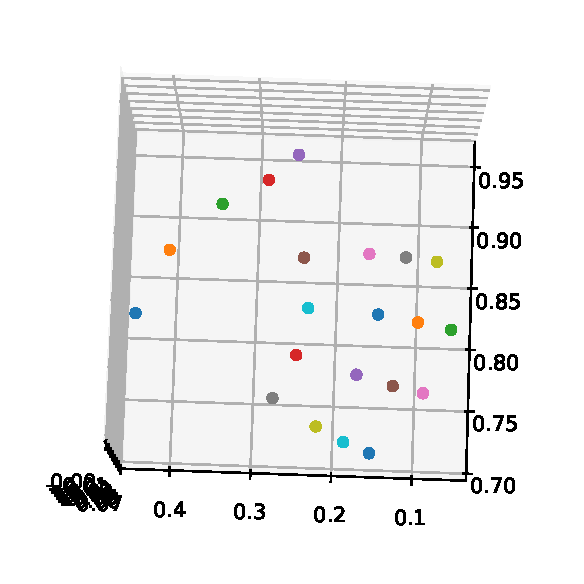
\includegraphics[width=0.8\linewidth]{slike/3D_coordinates.pdf}
    \caption{Отворена шака у 3Д простору.}
    \label{fig:slika3d}
\end{figure}

\begin{figure}[H]
    \centering
    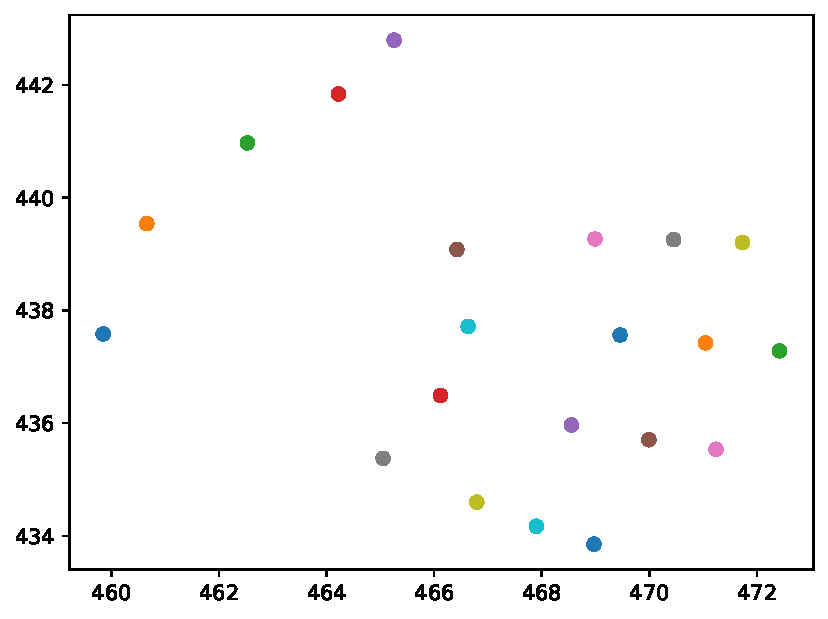
\includegraphics[width=0.8\linewidth]{slike/2D_coordinates.pdf}
    \caption{Отворена шака у 2Д простору.}
    \label{fig:slika2d}
\end{figure}

\subsection{Скуп података}

Скуп података система за препознавање гестикулација је направљен коришћењем CSV датотеке. Укупно садржи четрдесет три колоне. У првој колони су ознаке осам класа, односно осам гестикулација у опсегу од нула до седам. Остале четрдесет две колоне садрже редом $x$ и $y$ нормализоване координате кључних тачака шаке чије вредности су у опсегу од нула до један. Сваки ред дефинише један узорак, односно једну гестикулацију.  
  

\vspace{1em}

За сваку гестикулацију формирану десном шаком узета су по педесет два узорка, односно CSV датотека има по педесет два реда за сваку класу (0 - 7) формирану десном шаком. За сваку гестикулацију формирану левом шаком узета су такође по педесет два узорка. Скуп података укупно има осамсто тридесет два узорка, односно осамсто тридесет два реда.


\subsection{Класификација гестикулација}

Потпуно повезана неуронска мрежа за класификацију гестикулација дефинисана је методом \verb |neural_network()| из листинга~\ref{lst:py:network}. Неуронска мрежа има четири слоја, три скривена слоја и један излазни слој. Први скривени слој има двадесет неурона, други скривени слој има такође двадесет неурона, а трећи скривени слој има десет неурона. Излазни слој има осам неурона.

\begin{lstlisting}[language=Python, caption={Имплементација метода коришћених за класификацију гестикулација.}, label={lst:py:network}]
# following three lines are added per Copilot suggestion 
import os
os.environ['PYTHONHASHSEED'] = '0'
os.environ['TF_DETERMINISTIC_OPS'] = '1'

from tensorflow import keras
from keras.models import Sequential
from keras.layers import Dense
from numpy import loadtxt
from tensorflow.keras.optimizers import Adam
from tensorflow.keras.losses import SparseCategoricalCrossentropy
from tensorflow.keras.metrics import SparseCategoricalAccuracy
#from random import shuffle
from numpy.random import shuffle
from utils import save_model

import matplotlib.pyplot as plt
import numpy as np
import tensorflow as tf
import random

"""Sigmoid function is used for binary classification. Softmax is used for 
multi-class scenarios.
"""

SEED = 7

def split_data(data, mix, test_rate):
    
    if mix == True:
        shuffle(data)
    test_num = int(len(data)*(1 - test_rate))
    
    x_train = data[:test_num, 1:43]
    y_train = data[:test_num, 0]
    x_test = data[test_num:, 1:43]
    y_test = data[test_num:, 0]
    
    return x_train, y_train, x_test, y_test

def plot_history(history):
    """
    Plot training and validation accuracy and loss
    This method is added per Copilot suggestion 
    """
    fig, (ax1, ax2) = plt.subplots(1, 2, figsize=(12, 4))
    
    # Plot accuracy
    ax1.plot(history.history['sparse_categorical_accuracy'], label='Train Accuracy')
    ax1.plot(history.history['val_sparse_categorical_accuracy'], label='Test Accuracy')
    ax1.set_title('Model Accuracy')
    ax1.set_xlabel('Epoch')
    ax1.set_ylabel('Accuracy')
    ax1.legend()
    ax1.grid(True)
    
    # Plot loss
    ax2.plot(history.history['loss'], label='Train Loss')
    ax2.plot(history.history['val_loss'], label='Test Loss')
    ax2.set_title('Model Loss')
    ax2.set_xlabel('Epoch')
    ax2.set_ylabel('Loss')
    ax2.legend()
    ax2.grid(True)
    
    plt.tight_layout()
    plt.show()
    
def neural_network(x_train, y_train, x_test, y_test):
    
    model = Sequential()
    model.add(Dense(20, input_dim=42, activation='relu'))
    model.add(Dense(20, activation='relu'))
    model.add(Dense(10, activation='relu'))
    model.add(Dense(8, activation='softmax')) 
    
    model.compile(optimizer=Adam(),
                  loss=SparseCategoricalCrossentropy(),
                  metrics=[SparseCategoricalAccuracy()])
    
    model.summary()
    
    history = model.fit(x_train, y_train, epochs=100, validation_data=(x_test, y_test))
    
    return model, history

def main():
    
    # Set seeds at the beginning of main to ensure reproducibility
    random.seed(SEED)
    np.random.seed(SEED)
    tf.random.set_seed(SEED)
    
    dataset = loadtxt('dataset_8_both_hands.csv', delimiter=',')
    print(dataset)
    
    x_train, y_train, x_test, y_test = split_data(dataset, True, 0.2)
    
    model, history = neural_network(x_train, y_train, x_test, y_test)
    
    # Plot training history
    plot_history(history)
    
    _, accuracy = model.evaluate(x_train, y_train)
    print('Train accuracy: %.2f' % (accuracy*100))
    
    test_loss, test_acc = model.evaluate(x_test, y_test)
    print(f'\nTest accuracy: {test_acc}')
    
    filename="model_8_both_hands_19_1_v3.h5"
    save_model(model, filename)
        
if __name__ == "__main__":
    main()
\end{lstlisting}


\subsection{Тестирање система }

Метода \verb |evaluate()| \textit{Keras} библиотеке позвана у линијама 104 и 107 листинга~\ref{lst:py:network} коришћена је за процењивање тачности модела тј. система за препознавање гестикулација. Резултат извршавања ове методе приказан је у листингу~\ref{lst:py:testing1}. Метода \verb |plot_history()| приказана у листингу~\ref{lst:py:network} се користи за исцртавање графика приказаних на слици~\ref{fig:slikaaccloss}. 

\begin{figure}[H]
    \centering
    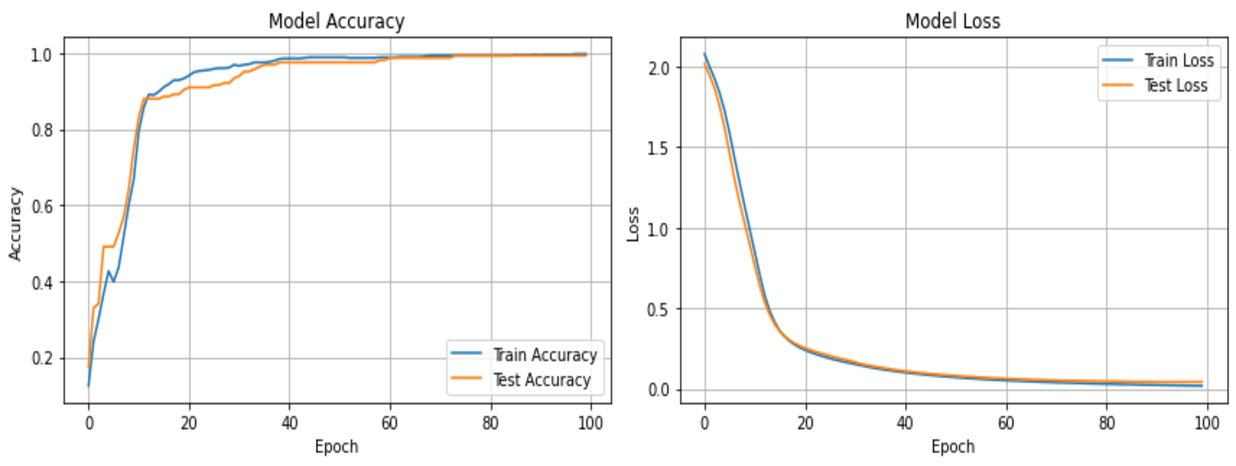
\includegraphics[width=\linewidth]{slike/Figure_final_model.pdf}
    \caption{Тачност и губитак на скупу за тренирање и скупу за тестирање }
    \label{fig:slikaaccloss}
\end{figure}

На графику лево функција приказана плавом бојом представља тачност модела на подацима за тренирање у зависности од епоха, а функција приказана наранџастом бојом представља тачност модела на подацима за тестирање у зависности од епоха.  На графику десно функција приказана плавом бојом представља губитак на подацима за тренирање у зависности од епоха, а функција приказана наранџастом бојом представља губитак на подацима за тестирање у зависности од епоха.

\begin{lstlisting}[caption={Резултат евалуације неуронске мреже на подацима за тренирање и тестирање.}, label={lst:py:testing1}, numbers=none, xleftmargin=6cm, frame=none]
Train accuracy: 99.85
Test accuracy: 99.40
\end{lstlisting}

На слици~\ref{fig:grecognition} приказан је прозор камере система за препознавање гестикулација у тренутку препознавања круга (енгл. \textit{ok}).


\begin{figure}[H]
    \centering
    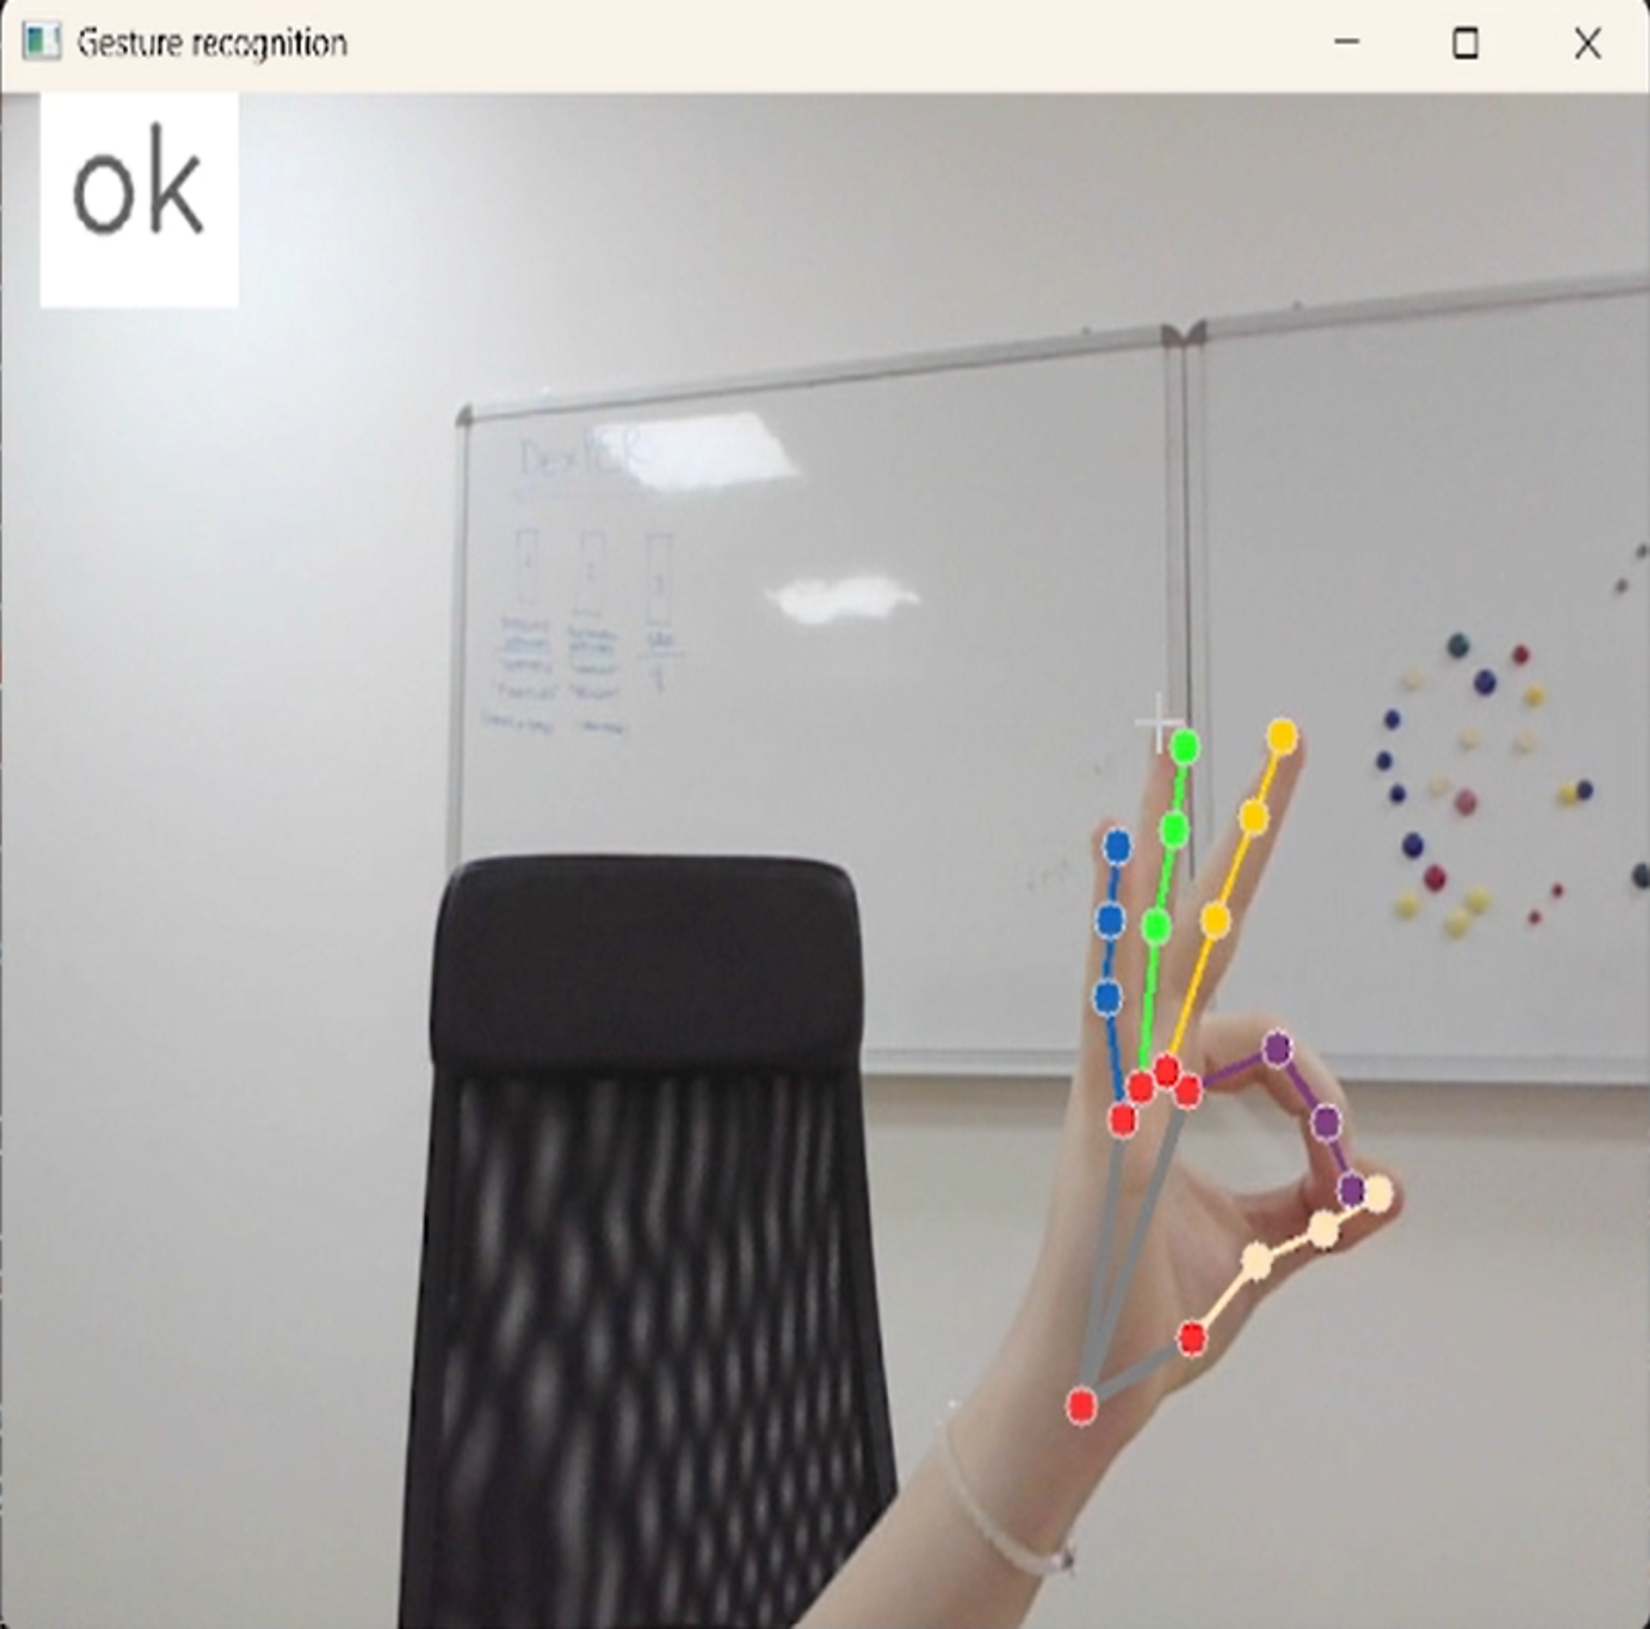
\includegraphics[width=0.9\linewidth,height=0.9\textheight,keepaspectratio]{slike/finalWindow.pdf}
    \caption{Прозор камере система за препознавање гестикулација.}
    \label{fig:grecognition}
\end{figure}

\subsubsection{Тест скуп података направљен од координата кључних тачака шака које нису коришћене за тренирање модела}

Претходно поменут, први тест скуп података је направљен од координата кључних тачака шака једне особе чије шаке су коришћене и за тренирање модела. Тај скуп података је добијен дељењем укупног скупа података на скуп за тренирање и скуп за тестирање.

Други тест скуп података, направљен од координата кључних тачака шака које нису коришћене за тренирање модела је прикупљен од шака друге особе.

\begin{lstlisting}[caption={Резултат евалуације модела неуронске мреже на другом тест скупу података.}, label={lst:py:testing2}, numbers=none, xleftmargin=6cm, frame=none]
Test accuracy: 88.02
\end{lstlisting}

\section{Закључак}

У оквиру овог рада имплементиран је систем за препознавање осам гестикулација шаком са тачношћу 99.4\% за особу чије шаке су коришћене и за тренирање неуронске мреже. Успешно је извршена пројекција 3Д координата кључних тачака шаке у 2Д координате коришћењем параметара добијених калибрацијом камере која је описана у поглављу 4. Добијени параметри су специфични за сваку камеру и одговарају искључиво веб камери рачунара који је коришћен за имплементацију овог система. Поред тестирања система коришћењем тест скупа података који је добијен поделом укупног скупа података састављеног од података једне особе на скуп за тренирање и скуп за тестирање узети су и узорци друге особе од којих је направљен други скуп података за тестирање. Тачност система за препознавање гестикулација добијена коришћењем поменутог скупа података друге особе чије шаке нису коришћене за тренирање неуронске мреже пада на 88.02\%. Укупан скуп података потпуно повезане неуронске мреже за класификацију гестикулација се састоји од 2Д координата кључних тачака шака само једне особе. Број узорака по гестикулацији није велики. За сваку гестикулацију формирану десном шаком узета су по педесет и два узорка и за сваку гестикулацију формирану левом шаком узета су такође по педесет и два узорка. Поменути број узорака може утицати на отпорност система на варијације и промене, односно на то како систем ради када корисник формира гестикулацију мало другачије и под различитим угловима камере.

Систем за препознавање гестикулација би могао да се унапреди додавањем података више особа, односно додавањем координата кључних тачака шака различитих величина, старости и полова у скуп података за тренирање неуронске мреже. При тестирању у реалном времену примећено је да систем понекад помеша једну од осам гестикулација, нпр. уместо затворене шаке формиране левом руком препознаје рокенрол знак док за исту гестикулацију формирану десном руком не прави ту грешку. Поменута тачност 99.4\% добијена на статичким подацима показује да су такве грешке очекиване и у реалном времену. Препорука за унапређење система за препознавање гестикулација је коришћење \textit{IPN HandS}~\cite{app15116321} алата и скупа података које предлажу истраживачи Gibran Benitez-Garcia, et al. (2025). \textit{IPN HandS} је побољшана верзија \textit{IPN Hand}~\cite{bega2020IPNhand} скупа података која обухвата приближно 700,000 примерака скелета шаке где је за сваки примерак дефинисана двадесет једна кључна тачка шаке. \textit{IPN Hand} скуп податакa садржи видео датотеке које је снимило педесет испитаника. Не садржи директно координате кључних тачака шака, али се из видео датотека координате могу добити коришћењем \textit{MediaPipe Hands} решења. Код \textit{IPN HandS} скупа података исправљени су и временски интервали гестикулација из видео снимака тј. почетни тренутак и крајњи тренутак сваке гестикулације у видео снимку. 

Систем предложен у овом мастер раду даље може да се надогради тако да поред статичких гестикулација препознаje и покрете. На тај начин би систем био способан да разуме и знаковни језик који зависи од покрета. Друштвена корист таквог система огледа се у томе што би њиме била решена комуникацијска баријера између глувих и наглувих особа које користе знаковни језик и већине људи који знаковни језик не разумеју. Систем би требало да буде способан да препозна знаковни језик и да га аутоматски преводи у текст или говор. Могао би да буде пројектован као мобилна апликација на паметним телефонима како би глуве и наглуве особе могле да га користе било где и било када.

\makebibliography

\end{document}